\documentclass[../master_thesis.tex]{subfiles}
\begin{document}
\section{Variational formulation of the magnetostatic problem in 2D} 

For simplicity we will now turn to the 2D case and we assume that 
our open domain will be bounded and Lipschitz. This involves introducing
a different Hilbert complex with other differential operators. Then we 
derive the 2D magnetostatic problem from the three-dimensional one. 
We will assume our domain $\Omega$ to have a "annulus like" form which we 
will clarify in more rigour. In order for the 2D magnetostatic problem to be well-posed 
we require an additional constraint that will again be a curve integral. 
We will investigate an alternative way to represent this curve integral 
which will turn out to be easily suitable to be included in our numerical 
approximation. Prerequisite for this section are knowledge about basic functional analysis 
and fundamentals of finite element theory. We will also depend on the 
notions introduced in Sec.\,\ref{}, in particular the Hodge decomposition in the general 
case.

\subsection{The $\veccurl$-$\diver$ Hilbert complex}\label{sec:variational_formulation_of_the_magnetostatic_problem_in_2D}


We start with the introduction of the relevant differential operators and 
the resulting 2D Hilbert complex. We will then explain what domains we will consider 
and state the magnetostatic problem in strong form.

We define the scalar curl for $\mathbf{v} \in C^1(\Omega;\real^2)$ as
\begin{align*}
    \curl \mathbf{v} = \partial_1 v_2 - \partial_2 v_1.
\end{align*}
Additionally, we have the vector-valued curl, denoted in bold, defined 
for $v \in C^1(\Omega)$
\begin{align*}
    \veccurl v = \begin{pmatrix}\partial_2 v \\ -\partial_1 v    \end{pmatrix}.
\end{align*}
The cross product for 2D reads for $\mathbf{a}, \mathbf{b} \in \real^2$,
\begin{align*}
    \mathbf{a} \times \mathbf{b} \vcentcolon= a_1 b_2- a_2 b_1 
    = \mathbf{a} \cdot \mathbf{R}_{-\pi/2}\mathbf{b}.
\end{align*}
where $\mathbf{R}_{-\pi/2}$ is the rotation in clockwise direction by $\pi/2$.

A straightforward calculation shows that the following integration-by-parts formula 
holds for $u \in C^1(\overline{\Omega})$, $\mathbf{v} \in C^1(\overline{\Omega};\real^2)$,
assuming $\Omega$ is Lipschitz and bounded
\begin{align}
    \int_\Omega \veccurl u \cdot \mathbf{v} \,dx 
    = \int_\Omega u \, \curl \mathbf{v} \, dx + \int_{\partial \Omega} u\, \mathbf{v} \times \mathbf{n} \, d\ell
    \label{eq:2D_integration_by_parts_curl}
\end{align}
where $\mathbf{n}$ is the outward unit normal of $\Omega$.
Analogous to what we did in Sec.\,\ref{sec:adjoints_differential_operators_3d} 
we can now extend this definition in the weak sense.
First, notice that $\veccurl u = R_{-\pi/2} \grad u$ and thus $\veccurl$ is well-defined 
on $H^1$. For the scalar curl we define 
\begin{align*}
    H(\curl;\Omega) = \{ \mathbf{v} \in L^2 \mid \exists  w \in L^2: 
        \int_\Omega w \phi \, dx = \int_\Omega \mathbf{v} \cdot \veccurl \phi \, dx 
        \quad \forall \phi \in C_0^\infty \}
\end{align*}
and we denote $w$ in the definition -- which is uniquely determined -- 
as $\curl \mathbf{v}$, so in short
$(\curl, H(\curl)) = (\veccurl, C_0^\infty)^*$. 
Analogous to Section\,\ref{sec:adjoints_differential_operators_3d}, it is then possible to extend the 
tangential trace to an operator $\gamma_\tau$ defined on $H(\curl)$ s.t. 
for any $u\in H^1(\Omega)$, $\mathbf{v} \in H(\curl)$
the integration by parts formula
\begin{align*}
    \langle \veccurl u, \mathbf{v} \rangle = \langle  u, \curl \mathbf{v} \rangle 
        + \langle \gamma_\tau \mathbf{v} , \tr u \rangle_{H^{-1/2}(\partial \Omega)\times H^{1/2}(\partial \Omega)}.
\end{align*}
holds. From now on we will leave out the subindex of the duality inner product. Also analogous to the 3D case,
we can define 
\begin{align*}
    H_0(\curl) \vcentcolon= \{ \mathbf{v} \in H(\curl) \mid \gamma_\tau \mathbf{v} = 0\}
\end{align*}
and can then compute the adjoints analogously to what we did in Section\,\ref{sec:adjoints_differential_operators_3d},
\begin{align*}
    (\curl, H_0(\curl)) & = (\veccurl, H^1)^* 
    \\ (\curl, H(\curl)) & = (\veccurl, H_0^1)^*.
\end{align*}

Notice that $\diver \veccurl = 0$ and so 
we have the following 2D Hilbert complex 
\begin{align}
    H^1_0 \xrightarrow{\veccurl} H_0(\diver) \xrightarrow{\diver} L^2. \label{eq:2D_hilbert_complex}
\end{align}
and the dual complex
\begin{align*}
    L^2 \xleftarrow{\curl} H(\curl) \xleftarrow{-\grad} H^1
\end{align*}
We use the notation introduced in Sec.\,\ref{sec:hilbert_complexes} for general Hilbert complexes i.e.
$V^0 = H^1_0$, $V^1= H_0(\diver)$, $V^2= L^2$, $V^*_0 = L^2$, $V^*_1 = H(\curl)$ $V^*_2 = H^1$, 
$d^0 = \veccurl$, $d^1 = \diver$ and we set $d^k=0$ for the remaining $k \in \mathbb{Z}$. 
$d^*_k$ is the adjoint of $d^k$.
Also we remind of 
the notation $\mathfrak{B}^k$ for the image of the differential operator, $\mathfrak{B}^*_k$ 
for the image of the adjoint and analogous $\mathfrak{Z}^k$ for the kernel and 
$\mathfrak{Z}_k^*$ for the kernel of the adjoint.

\begin{remark}
    Since we are working only on bounded domains in this and the coming sections, 
    the Hilbert complex is closed i.e. all the images of the differential operators 
    are closed subspaces w.r.t. the $V$-norm. This was stated in 
    Thm.\,\ref{thm:closed_range} for the three-dimensional case, but it holds 
    for 2D as well. This is because these are both special cases for the analogous result 
    for the exterior derivative on Riemannian manifolds 
    in arbitrary dimensions (see \cite[Sec.\,6.2.6]{arnold}). This means
    in particular that we can use the Poincaré inequality (Thm.\,\ref{thm:poincare_inequality}).
\end{remark}

\subsection{Strong formulation of the 2D magnetostatic problem}

The 2D magnetostatic problem will be derived from a special case of the 3D problem.
Then the type of domains considered will be clarified and the strong formulation 
stated at the end.

Assume that our current source 
$\mathbf{J}$ is pointing in $z$-direction i.e. $\mathbf{J} = J \mathbf{e}_3$. 
Further assume that there is a $\tilde{\Omega}$ s.t. 
$\Omega = \tilde{\Omega} \times \real$. If $B_3$ does not change in $z$-direction we get that 
\begin{align*}
    0 = \diver \mathbf{B} = \partial_x B_1 + \partial_y B_2 = \diver \tilde{\mathbf{B}}.
\end{align*}
where $\tilde{\mathbf{B}} = (B_1,B_2)^\top$. The third component of the equation
$\curl \mathbf{B} = \mathbf{J}$ from the magnetostatic problem reads 
\begin{align*}
    J = \partial_x B_2 - \partial_y B_1 = \curl \tilde{\mathbf{B}}
\end{align*}
For $\Omega$ the unit outer normal is zero in $z$-direction and thus $\tilde{\mathbf{B}}$ 
satisfies the boundary 
condition
\begin{align*}
    0 = \mathbf{B} \cdot \mathbf{n} = \tilde{\mathbf{B}} \cdot \tilde{\mathbf{n}}
\end{align*}
with $\tilde{\mathbf{n}} = (n_1, n_2)^\top$ being the outer unit normal 
$\tilde{\Omega}$. 

Now we will abuse notation and refer to $\tilde{\mathbf{B}}$ as $\mathbf{B}$, 
$\tilde{\mathbf{n}}$ as $\mathbf{n}$ and $\tilde{\Omega}$ as $\Omega$.
Let $J \in L^2$ be given. Then we see that $\mathbf{B}$ must fulfill the 
following equations
\begin{align*}
    \curl \mathbf{B} &= J,
    \\ \diver \mathbf{B} &= 0.
\end{align*}
Depending on the domain, this problem is in general not well-posed -- just as the problem in 3D -- 
and requires an additional constraint. Let us now make certain restrictions 
on what type of domain we will consider. 

From now on, we assume that the space of harmonic forms $\mathfrak{H}^1$ has dimension 
one and that our domain is encompassed by two disjoint closed curves
i.e. we have curves $\partial \Omega_{in}$ and $\partial \Omega_{out}$ s.t. 
$\partial \Omega_{in} \dot\cup \partial\Omega_{out}$ is the boundary of $\Omega$. 
Let now $\Gamma$ be s.t. it is a closed curve in $\Omega$ that goes around the 
hole in the middle i.e. the area surrounded by $\Gamma$ contains $\partial \Omega_{in}$.
Denote its parametrization with $\bm{\gamma}:[0,|\Gamma|] \rightarrow \Omega$ s.t. 
$|\bm{\gamma}'(t)| = 1$ and assume that $\bm{\gamma}$ is bijective i.e. the curve does not 
intersect itself. We assume that $\Gamma$ has positive distance from 
$\partial \Omega_{in}$. We do not assume anything like that for the exterior boundary 
i.e. $\Gamma$ can touch or be identical to $\partial \Omega_{out}$. 
We then denote the area that is enclosed by $\Gamma$ and
$\partial\Omega_{in}$ as $\Omega_\Gamma$ (cf. Fig.\,\ref{fig:annulus_domain}). 

\begin{figure}
    \centering
    \resizebox{8cm}{8cm}{
    \begin{tikzpicture}
    \draw[fill=lightgray] (0,0) circle [radius=5];
    \draw[fill=white] (0,0) circle [radius=2];
    \draw[dashed, -{Latex[length=3mm,width=3mm]}] (4,0) 
         arc [start angle=0, end angle=180, radius=4] node[midway, below]{\large$\Gamma$} ;
    \draw[dashed, -{Latex[length=3mm,width=3mm]}] (-4,0) arc [start angle=180, end angle=360, radius=4] ;
    \node[above] at (0,5) {\large$\partial \Omega_{out}$};
    \node[below] at (0,2) {\large$\partial \Omega_{in}$};
    \node at (135:3) {\huge$\Omega_\Gamma$};
\end{tikzpicture}
}
\caption{A simple example for a domain $\Omega$ as described. The boundary are two 
disjoint curves $\partial \Omega_{in}$ and $\partial \Omega_{out}$. The curve 
$\Gamma$ is parametrized in anticlockwise direction and $\Omega_\Gamma$ is the 
area enclosed by $\Gamma$ and $\partial \Omega_{in}$.} \label{fig:annulus_domain}
\end{figure}

From now on, our domain $\Omega$ is always assumed to be of that kind. We will 
later make further restrictions on what types of domain we will consider that 
will be suitable for discretization (see Assumption\,\ref{ass:discretizable_single_patch_domain}).


We add the curve integral along $\Gamma$, which we 
assume to be well-defined, as an additional constraint.
So in total, we obtain the following problem.
\begin{problem}[2D magnetostatic problem]\label{prob:2d_magnetostatic_problem}
    Given $J \in L^2$ and $C_0 \in \real$, find $\mathbf{B} \in H_0(\diver) \cap H(\curl)$ s.t.
    \begin{align*}
        \curl \mathbf{B} &= J, 
        \\ \diver \mathbf{B} &= 0,
        \\ \int_\Gamma \mathbf{B} \cdot \, dl &= C_0
    \end{align*}
\end{problem}

Another option for the additional constraint would be an orthogonality constraint as discussed 
in \cite[Sec.\,3.5]{multipatch_paper}.

\subsection{Mixed formulation}
In order to solve this problem numerically using finite elements, we have to 
choose a suitable variational formulation of the problem. This variational formulation 
will be stated without the curve integral constraint and then we will show 
the equivalence with the strong formulation.

Ignoring the curve integral 
at first, we will use the following. We choose a non-zero harmonic form 
$\mathbf{p} \in \mathfrak{H}^1$ and have 
$J \in L^2$ . Then the problem is: Find $\sigma \in H^1_0$, 
$B \in H_0(\diver)$ and $\lambda \in \real$ s.t.
\begin{align}
    \langle \sigma, \tau \rangle - \langle \mathbf{B}, \veccurl \tau \rangle 
        &=  -\langle J, \tau \rangle \quad \forall \tau \in H^1_0, \label{eq:first_eq_mixed_formulation}
    \\ \langle \veccurl\sigma, \mathbf{v} \rangle + \langle \diver \mathbf{B}, \diver \mathbf{v} \rangle 
        + \lambda \langle \mathbf{p}, \mathbf{v} \rangle 
        &= 0 \quad \forall \mathbf{v} \in H_0(\diver) \label{eq:second_eq_mixed_formulation}
\end{align} 
As before, the inner product without subscript denotes the $L^2$ inner product and 
$\lVert \cdot \rVert$ the $L^2$ norm.
Here the curve integral condition is missing. It is difficult to include the curve integral 
condition directly when solving this system numerically. So we will replace it below 
in Sec.\,\ref{sec:curve_integral_constraint}.

Even though this formulation appears more complicated in comparison to the first two equations of 
the 2D magnetostatic problem (Problem\,\ref{prob:2d_magnetostatic_problem}), 
it will turn out to be well-suited for finite element approximations.
But it begs the question if the two formulations are equivalent. We will first 
investigate the formulation without curve integral

\begin{proposition}
    For any $J \in L^2$, (\ref{eq:first_eq_mixed_formulation}) and 
    (\ref{eq:second_eq_mixed_formulation}) hold i.i.f. 
    $\sigma = 0$, $\lambda=0$, $\curl \mathbf{B} = J$ and 
    $\diver \mathbf{B} = 0$
    i.e. $\mathbf{B}$ solves the 2D magnetostatic problem (Problem\,\ref{prob:2d_magnetostatic_problem})  
    without the additional curve integral
    constraint.
\end{proposition}
\begin{proof}
    Assume $(\sigma,\mathbf{B},\lambda)$ is a solution of (\ref{eq:first_eq_mixed_formulation}) and 
    (\ref{eq:second_eq_mixed_formulation}). Then the first equation is
    \begin{align*}
        \langle \sigma + J, \tau \rangle  
        &=  \langle \mathbf{B}, \veccurl\tau \rangle  \quad \forall \tau \in H^1_0
    \end{align*}
    which is equivalent to $\mathbf{B} \in H(\curl)$ and $J + \sigma = \curl \mathbf{B}$.

    Now assume additionally, that  
    (\ref{eq:second_eq_mixed_formulation}) holds. Then by choosing $\mathbf{v} = \mathbf{p} \in \mathfrak{H}^1$,
    we get $\diver \mathbf{p} = 0$ from the definition of the harmonic forms 
    and $\mathfrak{H}^1 \perp \veccurl H^1_0$ from the Hodge decomposition and thus
    \begin{align*}
        \langle \veccurl \sigma, \mathbf{p} \rangle + \langle \diver \mathbf{B}, \diver\mathbf{p}\rangle 
            + \lambda\langle \mathbf{p}, \mathbf{p} \rangle
        = \lambda \langle \mathbf{p}, \mathbf{p}\rangle = 0
    \end{align*}
    and so $\lambda = 0$. Then we can choose $\mathbf{v} = \veccurl \sigma$ to get 
    \begin{align*}
        \langle \veccurl \sigma, \veccurl \sigma \rangle + \langle \diver \mathbf{B}, \diver \veccurl \sigma \rangle 
            + \lambda \langle \mathbf{p}, \veccurl \sigma \rangle
        = \lVert \veccurl \sigma \rVert^2 = 0.
    \end{align*}
    Because $\sigma \in H^1_0$ this gives us $\sigma = 0$. Also we have then 
    $J = \curl \mathbf{B}$. At last we choose $\mathbf{v} = \mathbf{B}$ which gives us 
    $\diver \mathbf{B} = 0$ and thus we proved the first direction. 

    The other implication is clear i.e. if $\mathbf{B} \in H(\curl) \cap H_0(\diver)$
    with $\curl \mathbf{B} = J$ and $\diver \mathbf{B} = 0$ then the variational 
    formulation clearly holds.
    \end{proof}
Notice that the variable $\lambda$ is not necessary for this variational formulation, 
but we will need it later, since we will add another equation representing the 
curve integral constraint and hence we need another variable to have the same 
number of unknowns and equations.
If we now add the same additional constraint to both formulations of the problem 
then they will remain equivalent.


\subsection{Curve integral constraint}\label{sec:curve_integral_constraint}

We still need to find a good way to include the curve integral constraint from 
Problem\,\ref{prob:2d_magnetostatic_problem} in our formulation. Instead of incorporating 
it directly, we will substitute it with another equation. We will first derive this 
equation as an immediate consequence of the integration by parts formula 
(\ref{eq:2D_integration_by_parts_curl}) and then state the 
final variational formulation of the 2D magnetostatic problem which we 
will investigate in the coming sections.

Because $\mathbf{n}$ is the unit outward normal 
of $\Omega_\Gamma$ and $\bm{\gamma}$ the parametrization of $\Gamma$ that $\mathbf{n} \perp \bm{\gamma}'$
and
\begin{align*}
    \mathbf{B}\times \mathbf{n} 
    = (B_1 n_2 - B_2 n_1) = \mathbf{B} \cdot \begin{pmatrix}n_2 \\ -n_1 \end{pmatrix}
    = -\mathbf{B} \cdot \mathbf{R}_{\pi/2}\mathbf{n}.
\end{align*}
$\mathbf{R}_{\pi/2} \mathbf{n}$ is either $\bm{\gamma}'$ or $-\bm{\gamma}'$. Assume w.l.o.g.
that $\mathbf{R}_{\pi/2} \mathbf{n} = \bm{\gamma}'$ and thus 
\begin{align*}
    \mathbf{B} \times \mathbf{n} = -\mathbf{B} \cdot \bm{\gamma}'
\end{align*}
and so the curve integral becomes

\begin{align*}
    \int_\Gamma \mathbf{B}\cdot d\ell= \int_0^{|\Gamma|} \mathbf{B}(\bm{\gamma}(t)) \cdot \bm{\gamma}'(t) \, dt 
    % = \int_0^{|\Gamma|} \mathbf{n}(\bm{\gamma}(t)) \times \mathbf{B}(\bm{\gamma}(t)) \, dt 
    = -\int_\Gamma  \mathbf{B}\times \mathbf{n} d\ell.
\end{align*}
Choose $\psi \in H^1$ s.t. $\psi = 0$ on $\partial \Omega_{in}$, $\psi = 1$ on 
$\partial \Omega_{out}$ and $\psi \equiv 1$ in $\Omega \setminus \Omega_\Gamma$
Then we observe 
\begin{align*}
    \int_\Omega \veccurl \psi \cdot \mathbf{B} \, dx = 
    \int_{\Omega_\Gamma} \veccurl \psi \cdot \mathbf{B} \, dx = 
    \int_{\Omega_\Gamma} \psi \, J \, dx + \int_{\partial\Omega} \mathbf{B} \times \mathbf{n}\, d\ell
    = \int_{\Omega_\Gamma} \psi \, J \, dx - \int_\Gamma \mathbf{B}\cdot d\ell
\end{align*}
So if the curve integral 
\begin{align*}
    \int_\Gamma \mathbf{B} \cdot d\ell = C_0
\end{align*}
is given and we can compute $\int_{\Omega_\Gamma} \psi \, J \, dx$
we can add the equation
\begin{align}
    \langle \veccurl \psi, \mathbf{B} \rangle = C_1 \label{eq:variational_curve_integral}
\end{align}
with 
\begin{align*}
    C_1 \vcentcolon= \int_{\Omega_\Gamma} \psi \, J \, dx - C_0
\end{align*}
to our system.

From the above derivations it is also clear that for $\mathbf{B} \in C^1(\overline{\Omega};\real^2)$ 
\begin{align*}
    \int_\Gamma \mathbf{B} \cdot d\ell = C_0 
    \Leftrightarrow \langle \veccurl \psi, \mathbf{B} \rangle = C_1.
\end{align*}
This is the motivation to add the right equation to our system instead
of the curve integral since it is much easier 
to enforce numerically.

In order to get a variational 
formulation to study theoretically,
 we multiply (\ref{eq:variational_curve_integral}) with an arbitrary $\mu \in \real$. 
In conclusion, we have the following variational problem:

\begin{problem}\label{prob:magnetostatic_problem_variational}
    Let $J \in L^2$, $\mathbf{p} \in \mathfrak{H}^1 \setminus \{0\}$. 
    Find $\sigma \in H^1_0$, $\mathbf{B} \in H_0(\diver)$, $\lambda \in \real$ s.t.
    \begin{align}
        \langle \sigma, \tau \rangle - \langle \mathbf{B}, \veccurl\tau \rangle 
        &=  -\langle J, \tau \rangle &&\quad \forall \tau \in H^1_0, \label{eq:first_eq_mixed_formulation_curve_integral}
        \\ \langle \veccurl\sigma, \mathbf{v} \rangle + \langle \diver \mathbf{B}, \diver \mathbf{v} \rangle 
        + \langle \lambda \mathbf{p}, \mathbf{v} \rangle 
        &= 0 &&\quad \forall \mathbf{v} \in H_0(\diver), \label{eq:second_eq_mixed_formulation_curve_integral}
        \\ \mu \langle \bm{\curl} \psi, \mathbf{B} \rangle &= \mu C_1 &&\quad \forall \mu \in \real.
    \end{align}
\end{problem}
\noindent which gives us the variational formulation of the magnetostatic problem with curve integral 
constraint (Problem\,\ref{prob:2d_magnetostatic_problem}). 
We will study the well-posedness of this formulation next. 

\subsection{Well-posedness of the magnetostatic system}\label{sec:well-posedness_of_magnetostatic_system}

The well-posedness is based on the well-known Banach-Nečas-Babuška (BNB) theorem 
concerning general variational problems of the following form: Find $x \in X$ 
s.t. 
\begin{align}
    a(x,y) = \ell(y) \quad \forall y \in Y \label{eq:general_variational_problem}
\end{align}
where $X$ and $Y$ are Banach spaces, $a$ is a bilinear form 
and $\ell \in Y'$. The BNB-theorem then answers the question of well-posedness 
i.e. if there exists a unique solution and if we can find a stability estimate.
The following formulation is from \cite[Sec.\,25.3]{ern_guermond_2} in the real case.

\begin{theorem}[BNB]\label{thm:BNB}
    Let $X$ be a Banach space and $Y$ be a reflexive Banach space. Let $a:X\times Y \rightarrow \real$ be a 
    bounded bilinear form and $\ell \in Y'$. Then a problem of the form 
    (\ref{eq:general_variational_problem}) is well-posed i.i.f. the following two criteria are fulfilled
    \begin{align}
        &\text{\normalfont(1)}\quad\inf_{x \in X} \sup_{y\in Y} \frac{|a(x,y)|}{\lVert x \rVert _X \lVert y \rVert _Y} 
            =\vcentcolon \gamma > 0\label{eq:BNB1} 
        \\&\text{\normalfont(2)}\quad \text{for any $y \in Y$ if $a(x,y) = 0$ for every $x \in X$, then $y=0$.}\label{eq:BNB2}
    \end{align}    
    We then obtain the stability estimate for a solution $x$
    \begin{align*}
        \lVert x \rVert _X \leq \frac{1}{\gamma} \lVert \ell\rVert _{Y'}.
    \end{align*}
\end{theorem}
Note that (\ref{eq:BNB1}) is equivalent to the fact that for any $x \in X \setminus\{0\}$ 
there exists $y \in Y\setminus\{0\}$ s.t. $a(x,y) \geq \gamma \lVert x \rVert _X \lVert y \rVert _Y$.  

Since we are dealing with Hilbert spaces only we can utilize the following proposition to prove it 
(see \cite[Rem.\,25.14]{ern_guermond}).
\begin{proposition}[$T$-coercivity]\label{prop:T_coercivity}
    Let $X$ and $Y$ be Hilbert spaces. Then {\normalfont (\ref{eq:BNB1})} and {\normalfont (\ref{eq:BNB2})} hold, if
    there exists a bounded bijective operator $T:X \rightarrow Y$ and $\eta >0$ s.t.
    \begin{align}
        a(x,Tx) \geq \eta \lVert x \rVert _X^2 \quad \forall x \in X. \label{eq:T_coercivity_bound}
    \end{align}
    Then $\gamma$ from {\normalfont (\ref{eq:BNB1})} can be chosen as $\eta/\lVert T \rVert  _{\mathcal{L}(X,Y)}$.
\end{proposition}
\begin{proof}
    For any $x \in X$, by taking $y = Tx \in Y$ and using the boundedness of 
    $T$ we have 
    \begin{align*}
        a(x,T(x)) \geq \eta \lVert x \rVert ^2 \geq \frac{\eta}{\lVert T \rVert  _{\mathcal{L}(X,Y)}}
            \lVert x \rVert _X \lVert y \rVert _Y
    \end{align*}
    and thus (\ref{eq:BNB1}) holds with $\gamma =  \frac{\eta}{\lVert T \rVert  _{\mathcal{L}(X,Y)}}$.

    For (\ref{eq:BNB2}) assume that we have $y \in Y$ s.t. $a(x,y) = 0$ for all 
    $x \in X$. 
    \begin{align*}
        0 = a(T^{-1}y,T T^{-1}y) \geq \eta \lVert T^{-1}y \rVert^2 _X
    \end{align*}
    so $T^{-1}y = 0$ and thus $y = 0$.
\end{proof}

\begin{remark}
    The other direction is also true i.e. if (\ref{eq:BNB1}) and (\ref{eq:BNB2}) 
    are fulfilled we can construct a $T$ with the desired properties.
\end{remark}

Note also that when we have found $T$ s.t. (\ref{eq:T_coercivity_bound}) holds 
then it must be injective. This is because if $Tx = 0$ for any 
$x \in X$ then $x=0$ follows from the $T$-coercivity.

The next step is to put our formulation of
Problem \ref{prob:magnetostatic_problem_variational} into 
this general framework. To this end, 
we define $X \vcentcolon= H^1_0 \times H_0(\diver) \times \real$
and for $(\sigma, \mathbf{B},\lambda) \in X$
\begin{align*}
    \lVert (\sigma, \mathbf{B}, \lambda) \rVert _X 
    \vcentcolon= \sqrt{\lVert \sigma \rVert^2_{H^1} + \lVert \mathbf{B} \rVert^2_{H(\diver)}
    + \lambda^2}.
\end{align*}
Notice that $X$ is then a Hilbert space with inner product 
\begin{align*}
    \langle (\sigma,\mathbf{B},\lambda), (\tau, \mathbf{v},\mu) \rangle _X 
    = \langle \sigma, \tau \rangle _{H^1} + \langle \mathbf{B}, \mathbf{v} \rangle _{H(\diver)} + \lambda \mu.
\end{align*}
For the formulation of the problem, we define the
bilinear form $a:X\times X \rightarrow \real$
\begin{align}
    a(\sigma,\mathbf{B}, \lambda;\tau,\mathbf{v},\mu) 
    =   \langle \sigma, \tau \rangle - \langle \mathbf{B}, \veccurl\tau \rangle
        + \langle \veccurl\sigma, \mathbf{v} \rangle + \langle \diver \mathbf{B}, \diver \mathbf{v} \rangle 
        + \langle \lambda \mathbf{p}, \mathbf{v} \rangle - \mu \langle \veccurl \psi, \mathbf{B} \rangle.
        \label{eq:definition_bilinear_form}
\end{align}
and 
\begin{align*}
    \ell(\tau,\mathbf{v},\mu) = -\langle J, \tau \rangle - \mu C_1.
\end{align*}
Then Problem\,\ref{prob:magnetostatic_problem_variational}
is equivalent to the following: Find $(\sigma,\mathbf{B},\lambda) \in 
X$ s.t.
\begin{align*}
    a(\sigma,\mathbf{B},\lambda;\tau,\mathbf{v},\mu) = \ell(\tau,\mathbf{v},\mu)
        \quad \forall (\tau,\mathbf{v},\mu) \in X.
\end{align*}
Note that the bilinear form $a$ is not symmetric. 

The next step is to show two important properties of $\veccurl \psi$ 
assuming $\psi$ has been chosen as described above.
\begin{proposition}
    Under the given assumptions on $\psi$, $\veccurl\psi \in H_0(\diver)$.
\end{proposition}
\begin{proof}
    We need to show $0 = \gamma_n \veccurl \psi$. Recall that the definition of 
    \begin{align*}
        \langle \gamma_n \veccurl \psi , \tr u \rangle 
        = \int_\Omega \veccurl \psi \cdot \grad u \, dx 
            + \int_\Omega \diver \veccurl \psi \, u \, dx 
    \end{align*}
    where the last term vanishes. Take now $\phi \in C^1(\overline{\Omega})$ 
    arbitrary. Then we take $\phi_1 \in C^1(\overline{\Omega})$ s.t. $\phi_1 = \phi$ in 
    a neighborhood of $\partial \Omega_{in}$ and zero near $\partial \Omega_{out}$. 
    Analogously, take $\phi_2 \in C^1(\overline{\Omega})$ s.t. $\phi_2 = \phi$ in 
    a neighborhood of $\partial \Omega_{out}$ and zero near $\partial \Omega_{in}$. Here we used the fact that 
    the two parts of the boundary are disjoint and have positive distance from one another.
    Then also $\tr \phi = \tr \phi_1 + \tr \phi_2$.
    We use the integration by parts formula from Thm.\,\ref{thm:trace_of_hdiv}, $\diver \veccurl = 0$ and the 
    integration-by-parts formula for the curl
    \begin{align*}
        &\langle \gamma_n \veccurl \psi , \tr \phi \rangle 
        = \langle \gamma_n \veccurl \psi , \tr \phi_1 \rangle + \langle \gamma_n \veccurl \psi , \tr \phi_2 \rangle
        \\ &= \int_\Omega \veccurl \psi \cdot \grad \phi_1 \, dx + \int_\Omega \veccurl \psi \cdot \grad \phi_2 \, dx
        \\ &= \int_\Omega \psi \cdot \curl \grad \phi_1 \, dx + \langle \gamma_\tau \grad \phi_1, \psi \rangle
            + \int_\Omega \psi \cdot \curl \grad \phi_2 \, dx + \langle \gamma_\tau \grad \phi_2, \psi \rangle.
    \end{align*}
    Here only the boundary terms remain because $\curl \grad =0$.
    Now remember that because $\phi_j \in C^1(\overline{\Omega})$, 
    $\langle \gamma_\tau \grad \phi_j, \psi \rangle 
    = \langle \grad \phi_j \times \mathbf{n}, \psi \rangle_{L^2(\partial \Omega)}$. So 
    \begin{align*}
        \langle \gamma_\tau \grad \phi_1, \psi \rangle 
        = \langle \grad \phi_1 \times \mathbf{n}, \psi \rangle_{L^2(\partial \Omega)} = 0
    \end{align*}
    because $\phi_1$ is zero near $\partial \Omega_{out}$ and $\psi$ is zero on 
    $\partial \Omega_{in}$. For the remaining term, 
    \begin{align*}
        \langle \gamma_\tau \grad \phi_2, \psi \rangle
        = \int_{\partial\Omega_{out}} \psi \grad \phi_2 \times \mathbf{n}d\ell 
        = \int_{\partial\Omega_{out}} \grad \phi_2 \times \mathbf{n} d\ell 
        = - \int_{\partial\Omega_{out}} \grad \phi_2 \cdot d\ell
    \end{align*}
    using a counter clockwise parametrization of $\partial\Omega_{out}$ 
    for a parametrization $\mathbf{s}$
    i.e. $\grad \phi_1 \times \mathbf{n} = -\grad \phi_1 \cdot \mathbf{R}_{\pi/2}\mathbf{s}'$
    and then we know from basic vector calculus because $\partial\Omega_{out}$ is closed
    \begin{align*}
        \int_{\partial\Omega_{out}} \grad \phi_1 \cdot d\mathbf{s} = 0.
    \end{align*}
    and so in conclusion, $\gamma_n \veccurl \psi = 0$.
\end{proof}

Usually the last equation in Problem\,\ref{prob:magnetostatic_problem_variational} 
is used to determine the harmonic part of the 
solution. This implies that we would like $\veccurl \psi$ to have 
non-vanishing harmonic part. This is indeed true.
\begin{proposition}
    Let $P_\mathfrak{H}^1: L^2 \rightarrow \mathfrak{H}^1$ be the orthogonal
    projection onto the harmonic forms. Then with $\psi$ defined as above 
    we have $P_\mathfrak{H}^1\veccurl \psi \neq 0$.
\end{proposition}
\begin{proof}
    Since $\diver \veccurl \psi = 0$ we know that 
    \begin{align*}
        \veccurl \psi \in \mathfrak{Z}^1 = \mathfrak{B}^1 \stackrel{\perp}{\oplus} \mathfrak{H}^1
    \end{align*}
    using the Hodge decomposition (cf. Thm.\,\ref{thm:hodge_decomposition}). 
    Assume for contradiction that $\veccurl \psi \in \mathfrak{B}^1$ i.e. there exists 
    $\psi_0 \in H^1_0$ s.t. $\veccurl \psi_0 = \veccurl \psi$. 
    Since $\veccurl$ is just the rotated gradient we would get that 
    $\grad (\psi - \psi_0) = 0$ and thus $\psi - \psi_0$ is constant almost 
    everywhere. But this is a contradiction since $\tr \psi_0$ is zero on $\partial\Omega_{in}$ 
    and $\partial \Omega_{out}$, but $\tr \psi = 0$ on $\partial\Omega_{in}$ and 
    $\tr \psi = 1$ on $\partial\Omega_{in}$. 
    Thus $\veccurl \psi \notin \mathfrak{B}^1$ and the claim follows.
\end{proof}
Now we can apply the Hodge decomposition of the $\ker \diver$ on
$\veccurl \psi$ and obtain the following
\begin{corollary}
    Let $\mathbf{p}\in \mathfrak{H}^1 \setminus \{ 0 \}$. Then there exists 
    $\psi_0 \in H^1_0$ and $c_\psi \in \real \setminus \{ 0 \}$ s.t. 
    \begin{align*}
        \veccurl \psi = \veccurl \psi_0 + c_\psi \mathbf{p}.
    \end{align*}
\end{corollary}
Because we can choose $\mathbf{p}$ we can assume w.l.o.g. that $c_\psi > 0$ and 
we will do so from now on.

As stated in the proof of the Poincare inequality (Thm.\,\ref{thm:poincare_inequality}), 
the $\veccurl| _{\mathfrak{Z}^\perp}: \mathfrak{Z}^\perp \rightarrow \mathfrak{B}^1$
is bijective and since it is bounded w.r.t. the $V$-norm -- which is the 
$H^1$-norm here -- due to Banach inverse theorem it is invertible and we denote this 
inverse $\veccurl^{-1}$. This is a slight abuse of notation since it is not really 
the inverse of the full $\veccurl$.

Let $P_\mathfrak{B}$ be the $L^2$-orthogonal projection onto $\mathfrak{B}^j$, 
we then denote $\mathbf{v}_\mathfrak{B} = P_\mathfrak{B} \mathbf{v}$ for any $\mathbf{v} \in L^2$ 
and analogous for 
$\mathfrak{H}^j$ and $\mathfrak{B}^*_j$.
In order to prove the $T$-coercivity, we need the following lemma.
\begin{lemma}\label{lem:T_for_T_coercivity_surjective}
    Take $\veccurl \psi = \veccurl \psi_0 + c_\psi \mathbf{p}$ with $c_\psi > 0$
    ,$\mathbf{p} \in \mathfrak{H}^1$ and $\lVert \mathbf{p}\rVert =1$.
    Define $T:X \rightarrow X$ as 
    \begin{align*}
        T(\sigma, \mathbf{B},\lambda)
        = (\sigma - \frac{1}{c_P^2}\veccurl^{-1}\mathbf{B}_\mathfrak{B}, \veccurl \sigma + \mathbf{B} + \lambda \beta \mathbf{p},
            \alpha \langle \mathbf{p}, \mathbf{B} \rangle  
            + \frac{\lambda}{c_\psi}).
    \end{align*}
    with $\alpha < 0$ and $\beta>0$.
    Then $T$ is bounded and surjective. 
\end{lemma}
\begin{proof}
    The boundedness is clear since all operators used in the definition 
    are bounded w.r.t. the norms of their domains. From the Poincaré inequality we know that 
    $\lVert \veccurl^{-1} \mathbf{B}_\mathfrak{B} \rVert \leq c_P \lVert \mathbf{B}_\mathfrak{B} \rVert$
    and so 
    \begin{align*}
        &\lVert T(\sigma,\mathbf{B},\lambda) \rVert^2 _X 
        = \lVert \sigma - \frac{1}{c_P^2}\veccurl^{-1}\mathbf{B}_\mathfrak{B} \rVert^2 _{H^1}
            + \lVert \veccurl \sigma + \mathbf{B} + \lambda \beta \mathbf{p} \rVert^2 _{H(\diver)}
             + \left( \alpha \langle \mathbf{p}, \mathbf{B} \rangle  + \frac{\lambda}{c_\psi} \right)^2
        \\ &\leq 2 \lVert \sigma \rVert ^2 _{H^1} 
            +  \frac{2}{c_P^4} \lVert \veccurl^{-1}\mathbf{B}_\mathfrak{B} \rVert ^2 _{H^1}
            + 3 \lVert \veccurl \sigma  \rVert^2 
            + 3 \lVert \mathbf{B} \rVert^2 _{H(\diver)}
            + 3 \lambda^2 \beta^2 + 2 \alpha^2 \lVert \mathbf{B}_\mathfrak{H}\rVert^2 
            + \frac{2}{c_\psi^2} \lambda^2
        \\ &\leq 2 \lVert \sigma \rVert ^2 _{H^1} 
            + \frac{2}{c_P^2} \lVert \mathbf{B}_\mathfrak{B} \rVert ^2 
            + 3 \lVert \veccurl \sigma  \rVert^2 
            + 3 \lVert \mathbf{B} \rVert^2 _{H(\diver)}
            + 3 \lambda^2 \beta^2 + 2 \alpha^2 \lVert \mathbf{B}\rVert^2 _{H(\diver)}
            + \frac{2}{c_\psi^2} \lambda^2
        \\ &\leq C_T \left( \lVert \sigma \rVert ^2 _{H^1} + \lVert \mathbf{B} \rVert^2 _{H(\diver)} 
            + \lambda^2 \right)
    \end{align*}
    with 
    \begin{align}
        C_T \vcentcolon= \max \left\{ 5, \frac{2}{c_P^2} + 3 + 2\alpha^2, 3 \beta^2 + \frac{2}{c_\psi^2} \right\}.
        \label{eq:bound_on_norm_of_T}
    \end{align}
    So $T$ is bounded and $\lVert T \rVert _{\mathcal{L}(X,Y)} \leq \sqrt{C_T}.$

    In order to prove surjectivity, we will split up $\mathbf{v} = \mathbf{v}_\mathfrak{B}
    + \mathbf{v}_\mathfrak{H} + \mathbf{v}_\mathfrak{B^*}$ using the Hodge decomposition.
    Take $(\tau, \mathbf{v},\mu) \in X$ arbitrary and 
    choose 
    \begin{align*}
        \sigma = (1+\frac{1}{c_P^2})^{-1} (\tau + \frac{1}{c_P^2} \veccurl^{-1} \mathbf{v}_\mathfrak{B}) 
        \text{ and }\mathbf{B}_\mathfrak{B} = \mathbf{v}_\mathfrak{B} - \veccurl \sigma.
    \end{align*}
    So 
    \begin{align*}
        \sigma -  \frac{1}{c_P^2} \veccurl^{-1}\mathbf{B}_\mathfrak{B} 
        = \sigma -  \frac{1}{c_P^2} (\veccurl^{-1} \mathbf{v}_\mathfrak{B} - \sigma)
        = (1+\frac{1}{c_P^2})\sigma - \frac{1}{c_P^2} \veccurl^{-1} \mathbf{v}_\mathfrak{B}
        = \tau.
    \end{align*}
    We simply choose $\mathbf{B}_\mathfrak{B^*} = \mathbf{v}_\mathfrak{B^*}$.
    For the harmonic part take $\kappa_v$ s.t. $\mathbf{v}_\mathfrak{H} = \kappa_v \mathbf{p}$.
    Let us look at the system 
    \begin{align*}
        \begin{pmatrix}
            1 & \beta 
            \\ \alpha & 1/c_\psi
        \end{pmatrix}
        \begin{pmatrix}
            \kappa_B 
            \\ \lambda 
        \end{pmatrix}
        = 
        \begin{pmatrix}
            \kappa_v 
            \\ \mu
        \end{pmatrix}
    \end{align*}
    Now since $c_\psi > 0$ and $\alpha < 0$, $\beta > 0$ we get 
    $1/c_\psi - \alpha \beta \neq 0$ and the system has a solution. 
    Choose $\mathbf{B}_\mathfrak{H} = \kappa_B \mathbf{p}$.
    Then we see 
    \begin{align*}
        \mathbf{v}_\mathfrak{H} = \kappa_v \mathbf{p} = \mathbf{p}(\kappa_B + \beta \lambda) 
        =  \mathbf{B}_\mathfrak{H} + \beta \lambda \mathbf{p}
    \end{align*}
    and 
    \begin{align*}
        \mu = \alpha \kappa_B + \frac{\lambda}{c_\psi}
        = \alpha \kappa_B \lVert \mathbf{p} \rVert^2 + \frac{\lambda}{c_\psi}
        = \alpha \langle \mathbf{B}, \mathbf{p} \rangle + \frac{\lambda}{c_\psi}.
    \end{align*}
    By combining all that we arrive at 
    $T(\sigma,\mathbf{B}, \lambda) = (\tau, \mathbf{v}, \mu)$.
\end{proof}

We assume from now on that we have always chosen $\mathbf{p}$ in a way s.t. 
$c_\psi$ -- as defined in the previous lemma -- is positive and $\mathbf{p}$ has 
norm one. This comes down to choosing $\mathbf{p}$ with the correct sign and normalizing it. 
Now we can use the T-coercivity (Prop.\,\ref{prop:T_coercivity}) to prove the inf-sup condition and thus 
well-posedness of our formulation.

\begin{theorem}
    Let $\veccurl \psi_0 + c_\psi \mathbf{p} = \veccurl \psi$ and assume we have chosen the sign of 
    $\mathbf{p}$ s.t. $c_\psi > 0$. Then take $c_1 >0 $ s.t. 
    $\lVert \veccurl \psi_0 \rVert \leq c_1$ (e.g. $c_1 = \lVert \veccurl \psi_0 \rVert + 1$ would be a valid choice). Define 
    $\beta = \frac{3 c_1^2 c_P^2}{c_\psi^2}$ and $\alpha = -\frac{c_\psi}{4 c_1^2 c_P^2}$. 
    Then the bilinear form $a$ defined at (\ref{eq:definition_bilinear_form}) 
    satisfies the inf-sup condition i.e. (\ref{eq:BNB1}) and (\ref{eq:BNB2})
    with $\gamma \geq \eta/\sqrt{C_T}$ with $C_T$ from (\ref{eq:bound_on_norm_of_T})
    and 
    \begin{align*}
        \eta \vcentcolon= \min \left\{ \frac{1}{2},  \frac{1}{4 c_P^2}, \frac{c_1^2 c_P^2}{c_\psi^2},
        \frac{c_\psi^2}{8 c_1^2 c_P^2}\right\}.
    \end{align*}
\end{theorem}
\begin{proof}
    We will use T-coercivity to prove it. Choose $(\sigma, \mathbf{B},\lambda) \in X$ 
    arbitrary and define $\rho \vcentcolon= \veccurl^{-1} \mathbf{B}_{\mathfrak{B}}$.
    We take $T$ as in (\ref{lem:T_for_T_coercivity_surjective}),
    \begin{align*}
        T(\sigma, \mathbf{B},\lambda)
        = (\sigma - \frac{1}{c_P^2}\rho, \veccurl \sigma + \mathbf{B} + \beta \lambda\mathbf{p},
            \alpha \langle \mathbf{p},\mathbf{B} \rangle  + \frac{\lambda}{c_\psi} )
    \end{align*}
    Then $T$ is surjective due to Lemma \ref{lem:T_for_T_coercivity_surjective}. 
    Note 
    \begin{align*}
        \langle \mathbf{B}, \mathbf{p} \rangle ^ 2
        = \lVert \mathbf{B}_\mathfrak{H} \rVert^2  
            \langle \frac{\mathbf{B}_\mathfrak{H}}{\lVert \mathbf{B}_\mathfrak{H} \rVert}, \mathbf{p} \rangle ^ 2
        = \lVert \mathbf{B}_\mathfrak{H} \rVert^2
    \end{align*}
    where we used in the last equality that $\frac{\mathbf{B}_\mathfrak{H}}{\lVert \mathbf{B}_\mathfrak{H} \rVert}$
    is either $+\mathbf{p}$ or $-\mathbf{p}$ because $\mathfrak{H}^1$ is assumed to be one-dimensional.
    We split up $\veccurl\psi = \veccurl\psi_0 + c_\psi \mathbf{p}$ to get 
    \begin{align*}
        &a(\sigma, \mathbf{B},\lambda;T(\sigma, \mathbf{B},\lambda))
        \\ &=\langle \sigma, \sigma - \frac{1}{c_P^2} \rho \rangle 
            - \langle \mathbf{B}, \veccurl \sigma - \frac{1}{c_P^2}\veccurl \rho \rangle
            + \langle \veccurl \sigma , \veccurl \sigma + \mathbf{B} + \beta \lambda \diver \mathbf{p} \rangle
        \\ &\quad + \langle \diver \mathbf{B}, \diver \veccurl \sigma 
            + \diver \mathbf{B} + \beta \lambda \diver \mathbf{p}\rangle
        \\ &\quad + \langle \lambda \mathbf{p}, \veccurl \sigma + \mathbf{B} + \beta \lambda \mathbf{p}\rangle
            - (\alpha \langle \mathbf{B}, \mathbf{p} \rangle + \frac{\lambda}{c_\psi})
            \langle \mathbf{B} , \veccurl\psi \rangle
        \\ &= \lVert \sigma \rVert^2 - \frac{1}{c_P^2} \langle \sigma , \rho \rangle 
            + \frac{1}{c_P^2} \lVert \mathbf{B}_\mathfrak{B} \rVert^2 + \lVert  \veccurl \sigma \rVert^2
            + \lVert \diver \mathbf{B} \rVert ^2 + \lambda ^2 \beta - \alpha c_\psi \lVert \mathbf{B}_\mathfrak{H} \rVert^2
        \\ &\quad- \alpha \langle \mathbf{p}, \mathbf{B}_\mathfrak{H} \rangle \langle \mathbf{B}_\mathfrak{B}, \veccurl \psi_0 \rangle
            - \frac{\lambda}{c_\psi} \langle \mathbf{B}_\mathfrak{B} , \veccurl \psi_0 \rangle
    \end{align*}
    Due to the Poincaré inequality
    \begin{align*}
        \lVert \rho \rVert \leq \lVert \rho \rVert _{H^1} 
        \stackrel{\text{Poincaré}}{\leq} c_P \lVert \veccurl \rho \rVert 
        = c_P \lVert \mathbf{B}_\mathfrak{B} \rVert.
    \end{align*}
    Using $\epsilon$-Young combined with Cauchy-Schwarz inequality several times 
    we obtain the lower bound.
    \begin{align*}        
        &\lVert \sigma \rVert^2 - 
            \left( \frac{1}{2} \lVert \sigma \rVert^2 
            + \frac{\lVert \mathbf{B}_\mathfrak{B} \rVert^2}{2 c_P^2}  \right)
            + \frac{1}{c_P^2} \lVert \mathbf{B}_\mathfrak{B} \rVert^2
            + \lVert  \veccurl \sigma \rVert^2 + \lVert \diver \mathbf{B} \rVert ^2
        \\ &\quad+ \lambda ^2 \beta - \alpha c_\psi \lVert \mathbf{B}_\mathfrak{H} \rVert^2
            - \left( \frac{\epsilon_1 \alpha^2 \lVert \mathbf{B}_\mathfrak{H} \rVert^2}{2} 
            + \frac{\lVert \mathbf{B}_\mathfrak{B} \rVert^2 \lVert  \veccurl \psi_0 \rVert^2}{2 \epsilon_1} \right)
            - \left( \frac{\lambda^2}{2 \epsilon_2 c_\psi^2} 
            + \frac{\epsilon_2 \lVert \mathbf{B}_\mathfrak{B} \rVert^2 \lVert  \veccurl \psi_0 \rVert^2}{2} \right)
    \end{align*}
    Choose $\epsilon_1 = 4 c_1^2 c_P^2$ to get 
    \begin{align*}
        &\frac{1}{2} \lVert \sigma \rVert^2 + \frac{1}{2 c_P^2} \lVert \mathbf{B}_\mathfrak{B} \rVert^2
        + \lVert  \veccurl \sigma \rVert^2 + \lVert \diver \mathbf{B} \rVert ^2
        + \lambda ^2 \left( \beta - \frac{1}{2 \epsilon_2 c_\psi^2} \right) 
        \\ &\quad+ \lVert \mathbf{B}_\mathfrak{H} \rVert^2 
        \left( - \alpha c_\psi - \frac{4 c_1^2 c_P^2 \alpha^2}{2} \right)
        - \lVert \mathbf{B}_\mathfrak{B} \rVert^2 \frac{\lVert  \veccurl \psi_0 \rVert^2}{8c_1^2 c_P^2}
        - \lVert \mathbf{B}_\mathfrak{B} \rVert^2 \frac{ \epsilon_2 \lVert  \veccurl \psi_0 \rVert^2 }{2}
    \end{align*}
    Now choose $\epsilon_2 = \frac{1}{4 c_1^2 c_P^2}$, plug in the definition of $\alpha$
    and use $\lVert \veccurl \psi_0 \rVert \leq c_1$ 
    to get the next lower bound
    \begin{align*}
        &\frac{1}{2} \lVert \sigma \rVert^2 + \lVert \mathbf{B}_\mathfrak{B} \rVert^2 
        \left( \frac{1}{2 c_P^2} - \frac{1}{8 c_P^2} 
        - \frac{\lVert  \veccurl \psi_0 \rVert^2}{8 c_1^2 c_P^2} \right)
        + \lVert  \veccurl \sigma \rVert^2 + \lVert \diver \mathbf{B} \rVert ^2
        + \lambda ^2 \left( \beta - \frac{4 c_1^2 c_P^2}{2 c_\psi^2} \right)
        \\ &\quad+ \lVert \mathbf{B}_\mathfrak{H} \rVert^2  \left( \frac{c_\psi^2}{4 c_1^2 c_P^2 }
        - \frac{ c_1^2 c_P^2 c_\psi^2}{8 c_1^4 c_P^4} \right)
    \end{align*}
    and finally by using the Poincaré inequality $\lVert \mathbf{B}_{\mathfrak{B}^*} \rVert 
    \leq c_P \lVert \diver \mathbf{B} \rVert$
    and $\beta = \frac{3 c_1^2 c_P^2}{c_\psi^2}$ we obtain the next bound
    \begin{align*}
        &\frac{1}{2} \lVert \sigma \rVert^2 + \frac{1}{4 c_P^2}\lVert \mathbf{B}_\mathfrak{B} \rVert^2 
            + \lVert  \veccurl \sigma \rVert^2
            + \frac{1}{2 c_P^2 } \lVert\mathbf{B}_{\mathfrak{B}^*}\rVert ^2
            + \frac{1}{2} \lVert \diver \mathbf{B} \rVert ^2
            + \frac{c_1^2 c_P^2}{c_\psi^2}\lambda^2
            + \frac{c_\psi^2}{8 c_1^2 c_P^2} \lVert \mathbf{B}_\mathfrak{H} \rVert^2.
        \\ &\geq \eta \lVert (\sigma,\mathbf{B},\lambda) \rVert^2_X 
    \end{align*}
    where we chose 
    \begin{align*}
        \eta \vcentcolon= \min \left\{ \frac{1}{2},  \frac{1}{4 c_P^2}, \frac{c_1^2 c_P^2}{c_\psi^2},
        \frac{c_\psi^2}{8 c_1^2 c_P^2}\right\} 
    \end{align*}
    to obtain the $T$-coercivity.
We can then choose $\gamma$ from (\ref{eq:BNB1}) as $\eta/\lVert T \rVert _{\mathcal{L}(X,X)}$
and then use $C_T$ from (\ref{eq:bound_on_norm_of_T}) to get a lower bound
\begin{align*}
    \gamma \geq \frac{\eta}{\sqrt{C_T}}. 
\end{align*}
\end{proof}

\begin{corollary}[Well-posedness]
    The variational formulation of the magnetostatic problem 
    {\normalfont (Problem\,\ref{prob:magnetostatic_problem_variational})} is well-posed. 
    For a solution $(\sigma, \mathbf{B},\lambda) \in X$
    we have the stability estimate 
    \begin{align*}
        \lVert \mathbf{B} \rVert  = \lVert (\sigma, \mathbf{B}, \lambda )\rVert _X 
        \leq \frac{\lVert J \rVert + |C_1|}{\gamma}.
    \end{align*}
\end{corollary}
\begin{proof}
    Recall that when $(\sigma, \mathbf{B},\lambda)$ is a solution 
    then $\sigma = 0$ and $\lambda = 0$ and $\diver \mathbf{B}=0$ which implies the 
    first equality.
    The statement follows immediately from the previous theorem and 
    Thm.\,\ref{thm:BNB} and the fact that 
    \begin{align*}
        | \ell(\tau,\mathbf{v},\mu) |
        = | - \langle J, \tau \rangle - C_1 \mu | 
        \leq (\lVert J \rVert + | C_1 |) \lVert (\tau,\mathbf{v},\mu) \rVert _X
    \end{align*}
    and thus $\lVert \ell \rVert _{X'} \leq \lVert J \rVert + | C_1 |$.
\end{proof}

\begin{remark}
    Note that $1/c_\psi$ terms arise
    in the stability constant $1/\gamma$. This is not surprising since the term 
    $\langle \veccurl \psi, \mathbf{B} \rangle$ will not enforce the harmonic 
    part if the harmonic part of $\veccurl \psi$ would be zero because 
    $\mathbf{B}_\mathfrak{H}$ will disappear from the formulation. So we 
    expect stability issues if the harmonic part is too small.
    This also forces us to choose $\psi$ with this in mind to obtain a 
    stable system.
\end{remark}

\section{Discretized magnetostatic problem}

In order to approximate solutions of the  2D magnetostatic problem we want to use finite elements.
A very typical question that arises for any discretization of a model is what 
notions of the continuous model are represented in the discretized one. 
In our case, a fundamental structure of our problem is the Hilbert complex we introduced in Section\,
\ref{sec:variational_formulation_of_the_magnetostatic_problem_in_2D}.
We would like to represent it in our discretization, leading to the discrete Hilbert complex. 
This section follows Sec. 5.2 in Arnold's book \cite{arnold}. We start with reviewing the 
general theory behind the discretization of general Hilbert complexes before applying this 
theory to our problem. Once we discretized our problem, we will utilize
the inf-sup condition proven in Section\,\ref{sec:variational_formulation_of_the_magnetostatic_problem_in_2D} 
to prove well-posedness of 
the discrete formulation and derive a quasi-optimal error estimate.

\subsection{Discrete Hilbert complex}\label{sec:discrete_hilbert_complex}

Let us at first stick to the general situation. We assume that we have a Hilbert complex 
$(W^k,d^k)$ with its corresponding domain complex 
$(V^k,d^k)$ and dual complex $(V^*_k,d^*_k)$ for $k \in \integers$. For this chapter 
we will only need a short subsequence 
\begin{align*}
    V^{k-1} \xrightarrow{d^{k-1}} V^k \xrightarrow{d^{k}} V^{k+1}
\end{align*}
for some fixed $k$ and $j \in \{k-1,k,k+1\}$ will always be the index to refer to 
all three spaces. We will sometimes leave out the indices if the meaning is clear from the context.

Let us assume that we have finite dimensional subspaces $V_h^j \subseteq V^j$. 
As usual in numerical analysis, $h>0$ stands loosely for the fineness of our discretization, 
e.g. the grid size or the maximal diameter of the elements in the mesh.
Then we define completely analogous to the continuous case,
\begin{align*}
    \mathfrak{Z}_h^j &\vcentcolon= \{ v_h \in V_h^j \mid d^j v_h = 0 \} = \ker d^j \cap V^j_h
    \\ \mathfrak{B}^j_h &\vcentcolon= \{ d^j v_h \mid v_h \in V_h^{j-1} \}.
\end{align*}
We can now also define the discrete harmonic forms. Now the situation is slightly 
different however. We will not use the adjoint $d^*_j$ to define it.
Instead,
\begin{align*}
    \mathfrak{H}_h^j \vcentcolon= \{ v \in \mathfrak{Z}_h^j \mid v \perp \mathfrak{B}^j_h \}
        = \mathfrak{Z}_h^j \cap \mathfrak{B}_h^{j,\perp}.
\end{align*}
Notice that we have $\mathfrak{Z}_h^j \subseteq \mathfrak{Z}^j$ and 
$\mathfrak{B}_h^j \subseteq \mathfrak{B}^j$, but due to 
$\mathfrak{B}_h^{j,\perp} \supseteq \mathfrak{B}^{j,\perp}$ we have in general
\begin{align*}
    \mathfrak{H}^j_h = \mathfrak{Z}_h^j \cap \mathfrak{B}_h^{j,\perp} 
    \not\subseteq    \mathfrak{Z}^j \cap \mathfrak{B}^{j,\perp} = \mathfrak{H}^j.
\end{align*}
We will later investigate the difference between the space of the discrete and continuous 
harmonic forms more closely.

There are three crucial assumptions that are necessary for stability and convergence 
of the method. The first one is the common and reasonable assumption that 
-- as usual in finite element theory -- we want that the discrete spaces $V_h^j$
 approximate the continuous ones $V^j$. 
\begin{assumption}\label{ass:convergence_discrete_spaces}
    For the discrete spaces, we require $V_h^j \subseteq V^j$ and
    \begin{align*}
        \lim_{h \rightarrow 0} \inf_{v_h \in V_h^j} \lVert w - v_h \rVert _V= 0, \quad \forall w \in V^j.
    \end{align*}    
\end{assumption}
This is usually satisfied for a reasonable choice of finite element space.
The next property is more restrictive and is a compatibility condition between the spaces.

\begin{assumption}
    For $j = k-1, k$,
    \begin{align*}
        dV_h^j \subseteq V_h^{j+1}.
    \end{align*}    
\end{assumption}
This means that we cannot simply use arbitrary 
discrete subspaces independent from one another. This property has a very nice
consequence. 
It shows that 
\begin{align*}
    V_h^{k-1} \xrightarrow{d^{k-1}} V_h^k \xrightarrow{d^k} V_h^{k+1}
\end{align*}
is itself a Hilbert complex and we can apply the general theory from 
Sec. \ref{sec:hilbert_complexes} directly to it. Let us do that.

Denote the restriction of $d^j$ to $V_h^j$ as $d_h^j$. Then as a linear map 
between finite spaces the adjoint -- denoted as $d_{j,h}^*: V_h^j \rightarrow V_h^{j-1}$ -- 
is everywhere defined. It is important to notice that in contrast to $d^j_h$ 
the adjoint $d^*_{j,h}$ is not the restriction of the adjoint $d^*_j$.
In general, $V^j_h \not\subseteq V_j^*$ and so the continuous adjoint might not be 
well-defined for a given $v_h \in V^j_h$. 

So we obtain the Hilbert complex
\begin{align}
    V_h^{k-1} \xrightarrow{d^{k-1}} V_h^{k} \xrightarrow{d^{k}} V_h^{k+1}\label{eq:discrete_hilbert_complex}
\end{align}
and its dual complex
\begin{align*}
    V_h^{k-1} \xleftarrow{d^*_{k,h}} V_h^{k} \xleftarrow{d^*_{k+1,h}} V_h^{k+1}
\end{align*}
From the general Hilbert complex theory (Thm.\,\ref{thm:hodge_decomposition})
we thus obtain the \textit{discrete Hodge decomposition}
\begin{align*}
    V_h^j = \mathfrak{B}^j_h \stackrel{\perp}{\oplus} \mathfrak{H}^j_h \stackrel{\perp}{\oplus}
        \mathfrak{B}^*_{jh}.
\end{align*}
So we achieved our goal of getting a structure like in the continuous case 
for our discrete approximation. We  will investigate the question how well the discrete harmonic 
forms approximate the continuous ones more thoroughly later.


\begin{assumption}
    There exist  \textit{bounded cochain projections} $\Pi^j_h : V^j \rightarrow V^j_h$. 
    This is a projection that is a cochain map in the sense of cochain complexes 
    (see Sec.\,\ref{sec:cohomology_groups}) i.e. 
    the following diagram commutes: 
    \\
    \begin{tikzcd}
    V^{k-1} \arrow[d, "\Pi^{k-1}_h"] \arrow[r, "d^{k-1}"] 
        & V^{k} \arrow[d, "\Pi^{k}_h"] \arrow[r, "d^{k}"] & V^{k+1} \arrow[d, "\Pi^{k+1}_h"]
    \\ V^{k-1}_h \arrow[r, "d^{k-1}"] & V^{k}_h  \arrow[r, "d^{k}"]& V^{k+1}_h 
    \end{tikzcd}
    \\   
    $\Pi^j_h$ are either bounded in the $V$- or in the $W$-norm. 
\end{assumption}
The cochain projection will play an important 
role in the stablity of the discrete system. 
Thanks to the commuting property, if $\Pi^j_h$ are $W$-bounded then they are $V$-bounded. 
In this section, we will make 
the weaker assumption of $V$-boundedness.

The fact that $\Pi_h$ is a $V$-bounded projection immediately allows a quasi 
optimal estimate. For any $v \in V^j$,  we can take 
$w_h \in V^j_h$ arbitrary s.t.
\begin{align}
    \lVert v - \Pi^j_h v \rVert _V
    &=  \lVert v - w_h  + \Pi^j_h  (w_h - v) \rVert _V
    \\ &\leq \lVert I - \Pi^j_h\rVert _{\mathcal{L}(V,V)} \lVert v - w_h \rVert _V. 
    \label{eq:bound_projection}
\end{align}
From now on we will denote the operator norm $\lVert \cdot \rVert _{\mathcal{L}(V,V)}$ 
by slight abuse of notation as $\lVert \cdot \rVert _V$.
Since $w_h$ was arbitrary we can take the infimum over $w_h \in V_h^k$ and obtain 
a quasi optimal estimate. 
% If we have the standard situation that 
% we have for $v \in V^j$
% \begin{align*}
%     \lVert v - \Pi^j_h v \rVert _V \leq C \lVert v  \rVert _V h^s
% \end{align*}
% for some generic constant $C>0$ independent of $v$ and the mesh size $h$ and some 
% $s>0$ then this implies 

Let us now answer the question about the difference between discrete and continous 
harmonic forms. In order to do that, we need some way to measure the "difference" 
between two subspaces. 

For a general metric space $(X,d)$, we will use the standard notation 
$d(x,M) \vcentcolon= \inf_{m\in M} d(x,m)$ for $x\in X$ being in a 
metric space and $M \subseteq X$. If we are dealing with a normed space then we 
take the metric induced by the norm.

\begin{definition}[Gap between subspaces]
    For a Banach space $W$ with subspaces $Z_1$ and $Z_2$
    let $S_1$ and $S_2$ be the unit spheres in $Z_1$ and $Z_2$ respectively i.e.
    $S_1 = \{ z\in Z_1 \mid \lVert z \rVert _W = 1 \}$ and analogous for $S_2$.
    Then we define 
    the gap between these subspaces as 
    \begin{align*}
        \gap(Z_1, Z_2) = \max\{ \sup_{z_1 \in S_1} d(z_1, Z_2), \sup_{z_2 \in S_2} d(z_2, Z_1) \}
    \end{align*}
\end{definition}
This definition is from \cite[Ch.4 §2.1]{kato_perturbation_theory} and defines a metric on the set of closed subspaces
of $W$.
If $W$ is a Hilbert space -- as it is throughout this section -- and $Z_1$ and $Z_2$ are closed then
the $\gap(Z_1, Z_2) = \lVert P_{Z_1} - P_{Z_2} \rVert _{\mathcal{L}(W,W)}$ i.e. the difference in operator norm of the 
orthogonal projections onto $Z_1$ and $Z_2$. This gives us a measure of distance between 
spaces which we can now apply to the question about the difference between 
discrete and continuous harmonic forms.

\begin{proposition}[Gap between harmonic forms]
    Assume that the discrete complex (\ref{eq:discrete_hilbert_complex}) admits a $V$-bounded cochain projection
    $\Pi_h$. Then
    \begin{align}
        \lVert (I - P_{\mathfrak{H}^k_h}) q \rVert _V \leq \lVert (I - \Pi_h^k) q \rVert _V, 
            \forall q \in \mathfrak{H}^k \label{eq:difference_identity_projection_discrete_harmonics}
        \\ \lVert (I - P_{\mathfrak{H}^k}) q_h \rVert _V 
        \leq \lVert (I - \Pi_h^k)P_{\mathfrak{H}^k} q_h \rVert _V, \quad 
                \forall q_h \in \mathfrak{H}^k_h 
    \end{align}
    and then 
    \begin{align*}
        \gap (\mathfrak{H}, \mathfrak{H}_h) 
        \leq \sup_{q \in \mathfrak{H}, \lVert q \rVert = 1} \lVert (I - \Pi_h^k) q \rVert _V
    \end{align*}
\end{proposition}
\begin{proof}
    See \cite[Thm.\,5.2]{arnold}. 
\end{proof}
The following proposition 
clarifies how close a discrete harmonic form can be chosen. But in order to prove it, 
we will need a small lemma.

\begin{lemma}\label{lem:distance_unit_sphere_whole_space}
    Let $W$ be a Banach space, $Z \subseteq W$ a closed subspace. Denote 
    $S_Z \vcentcolon= \{ z \in Z \mid \lVert z \rVert _W = 1 \}$. Then for 
    any $w \in W$ with $\lVert w \rVert _W = 1$ we get 
    \begin{align*}
        d(w,S_Z) \leq 2 \,d(w,Z)
    \end{align*}  
\end{lemma}
\begin{proof}
    See \cite[Ch.4 §2, (2.13)]{kato_perturbation_theory}.
\end{proof}

\begin{proposition}\label{prop:choice_of_discrete_harmonic_form}
    Take $p \in \mathfrak{H}^k$ with $\lVert p \rVert = 1$. Then we can 
    choose $p_h \in \mathfrak{H}_h^k$ with $\lVert p_h \rVert = 1$ s.t. 
    \begin{align*}
        \lVert p - p_h \rVert
        \leq 2\,\lVert I - \Pi_h^k\rVert _V \inf_{v_h \in V_h} \lVert p - v_h \rVert _V.
    \end{align*}
\end{proposition}
\begin{proof}
    Notice that since $\mathfrak{H}^k \subseteq \mathfrak{Z}^k$ we always have
    $\lVert q \rVert _V = \lVert q \rVert$ for all $q \in \mathfrak{H}^k$. The same is 
    true for $\mathfrak{H}^k_h$.
    Denote $S_h \vcentcolon= \{ q_h \in \mathfrak{H}^k_h \mid \lVert q_h \rVert = 1 \}$.
    Since $S_h$ is closed we can find $p_h \in S_h$ s.t. 
    \begin{align*}
        \lVert p_h - p \rVert = \inf_{q_h \in S_h} \lVert q_h - p \rVert
    \end{align*}
    The right hand side can be estimated using (\ref{eq:difference_identity_projection_discrete_harmonics}) 
    and then the 
    quasi optimal bound for the projection derived at (\ref{eq:bound_projection}).
    \begin{align*}
        \inf_{q_h \in S_h} \lVert q_h - p \rVert _V 
        &= \inf_{q_h \in S_h} \lVert q_h - p \rVert 
        \stackrel{\text{Lem.\,\ref{lem:distance_unit_sphere_whole_space}}}{\leq} 
            2\,\inf_{q_h \in \mathfrak{H}_h} \lVert q_h - p \rVert
        = 2\,\lVert P_{\mathfrak{H}_h}p - p \rVert
        \stackrel{(\ref{eq:difference_identity_projection_discrete_harmonics})}{\leq} 
            2\,\lVert \Pi_h^k p - p \rVert _V 
        \\ &\leq 2\,\lVert I - \Pi_h^k\rVert _{\mathcal{L}(V,V)}
            \inf_{v_h \in V_h} \lVert p - v_h \rVert _V
    \end{align*}
    which gives us the estimate.
\end{proof}

If we have the standard situation that 
we have for $v \in V^j$
\begin{align}
    \lVert v - \Pi^j_h v \rVert _V \leq C \lVert v  \rVert _V h^s \label{eq:standard_estimate_projection_error}
\end{align}
for some generic constant $C>0$ independent of $v$ and the mesh size $h$ and some 
$s>0$ then we can improve the estimate to
\begin{align*}
    \lVert p_h - p \rVert \leq C h^s
\end{align*}
by applying it in the last estimate of the proof.

Also if we assume $\lVert \Pi_h \rVert \leq c_\Pi$ for $h$ small enough and 
$c_\Pi > 0 $ independent of $h$ then we Assumption \ref{ass:convergence_discrete_spaces} implies
\begin{align*}
    p_h \xrightarrow{V} p \text{ as } h \rightarrow 0.
\end{align*}

\begin{theorem}[Dimension of $\mathfrak{H}^k_h$]\label{thm:dim_of_discrete_harmonic_space}
    Assume that we have a finite-dimensional subcomplex
    with a $V$-bounded cochain projection. Assume further, that 
    \begin{align}
        \lVert q - \Pi_h^k q \rVert < \lVert q \rVert, \quad \forall q \in \mathfrak{H}^k\setminus \{0\}.
        \label{eq:assumption_same_dimension}
    \end{align}
    Then $\mathfrak{H}^k$ and $\mathfrak{H}^k_h$ are isomorphic. 
    In particular, $\dim \mathfrak{H}^k = \dim \mathfrak{H}^k_h$.
\end{theorem}
\begin{proof}
    See \cite[Thm\,5.1]{arnold} and the explanation after the proof.
\end{proof}
If we assume a standard error estimate for the projection as (\ref{eq:standard_estimate_projection_error})
then (\ref{eq:assumption_same_dimension}) is fulfilled if $C h^s < 1$ which will be true 
for $h$ small enough.

\begin{proposition}\label{prop:gap_image_spaces}
    Assuming again a finite-dimensional subcomplex with a $V$-bounded cochain projection. 
    Then we can bound the gap between the image spaces
    \begin{align*}
        \gap (\mathfrak{B}^j_h, \mathfrak{B}^j) 
        \leq \lVert I - \Pi_h^j \rVert _V  \sup_{\substack{z \in \mathfrak{B}^j \\ \lVert z \rVert = 1} } 
        \inf_{v_h \in V^j_h} \lVert z - v_h \rVert _V.
    \end{align*}
\end{proposition}
\begin{proof}
    At first note, that for any $z \in \mathfrak{B}$, $\lVert z \rVert _V = \lVert z \rVert$.
    Since $\mathfrak{B}_h \subseteq \mathfrak{B}$, $d(z_h, \mathfrak{B}) = 0$ for any 
    $z_h \in \mathfrak{B}_h$. 
    
    Take $z \in \mathfrak{B}^j$ arbitrary i.e. there exists $w \in V^{j-1}$ s.t. 
    $dw = z$.
    Since $\Pi_h$  is a cochain projection, we thus have 
    \begin{align*}
        \Pi_h z = \Pi_h dw = d \Pi_h w \in \mathfrak{B}_h^j
    \end{align*}
    so $\Pi_h$ maps $\mathfrak{B}^j$ into $\mathfrak{B}^j_h$. Putting all that together,
    \begin{align*}
        d(z,\mathfrak{B}^j_h) = \inf_{z_h \in \mathfrak{B}_h} \lVert z - z_h \rVert 
        \leq \lVert z - \Pi_h z \rVert 
        = \lVert z - \Pi_h z \rVert _V
        \stackrel{(\ref{eq:bound_projection})}{\leq} \lVert I - \Pi_h \rVert _V \inf_{v_h \in V_h} \lVert z - v_h \rVert _V
    \end{align*}
    and then the claim follows from the definition of the gap.
\end{proof}

\begin{proposition}[Discrete Poincare inequality]
    Assume that we have a $V$-bounded cochain projection $\Pi_h$ for 
    the discrete Hilbert complex. Then 
    \begin{align*}
        \lVert v_h \rVert _V \leq c_{P,h}  \lVert dv_h \rVert, 
            \quad \forall v_h \in \mathfrak{Z}_h^{k\perp}\cap V_h
    \end{align*}
    with $c_{P,h} \vcentcolon= c_{P} \lVert \Pi_h \rVert _V$  and $c_P$ being the Poincare constant from 
    Thm.\,\ref{thm:poincare_inequality}.
\end{proposition}
\begin{proof}
    This indeed is a direct consequence of the existence of bounded cochain projections.
    Take $v_h \in \mathfrak{Z}_h^{k\perp}\cap V_h$ arbitrary. 
    Since $d (\mathfrak{Z}^{k,\perp} \cap V^k) = \mathfrak{B}^{k+1} \supseteq \mathfrak{B}^{k+1}_h$ we find 
    $z\in \mathfrak{Z}^{k\perp}\cap V_h$ s.t. $dz = dv_h$. We can apply now the continuous 
    Poincare inequality (Thm.\,\ref{thm:poincare_inequality}) to get $\lVert z \rVert _V \leq c_P \lVert dz \rVert _V = c_P \lVert dv_h \rVert _V$.
    Now we can use the fact that $\Pi_h$ is a cochain map 
    and the fact that $\Pi_h$ is a projection:
    \begin{align*}
        d\Pi^k_h z = \Pi^{k+1}_h dz = \Pi^{k+1}_h dv_h = dv_h
    \end{align*}
    For the last equality we used also the fact that we have a discrete complex i.e. $d^k V^k_h \subseteq V^{k+1}_h$.
    That shows that $d(v_h - \Pi_h z) = 0$ i.e. $(v_h - \Pi_h z) \in \mathfrak{Z}_h^k$.
    Because $v_h \in \mathfrak{Z}_h^{k,\perp}$ by assumption we have 
    \begin{align*}
        0 = \langle v_h, v_h - \Pi_h z \rangle = \langle v_h, v_h - \Pi_h z \rangle + \langle dv_h, d(v_h - \Pi_h z) \rangle
            = \langle v_h, v_h - \Pi_h z \rangle _V
    \end{align*}
    so $v_h - \Pi_h z$ is $V$ orthogonal to $v_h$. So 
    \begin{align*}
        \lVert v_h \rVert _V^2 &= \langle v_h, \Pi_h^k z \rangle _V + \langle v_h, v_h - \Pi_h^k z\rangle _V 
        = \langle v_h, \Pi_h^k z \rangle _V \leq \lVert v_h \rVert _V \lVert \Pi_h \rVert _V \lVert z \rVert 
        \\ &\stackrel{\text{Poincare ineq.}}{\leq} \lVert v_h \rVert _V c_P \lVert \Pi_h \rVert _V 
            \lVert dv_h \rVert _V
    \end{align*}
\end{proof}

Notice that if we assume that $\lim_{h \rightarrow 0} \lVert \Pi_h \rVert _V = 1$ 
(which is true if e.g. the standard estimate (\ref{eq:standard_estimate_projection_error}) is fulfilled)
then $c_{P,h} \rightarrow c_P$ for $h \rightarrow 0$.

In conclusion, we obtain a discrete version of the Hilbert complex where the harmonic forms are 
accurately represented if $h$ is small enough.

\subsection{Discretized magnetostatic problem}

Let us apply the theory of discrete Hilbert complexes to the 2D Hilbert complex (\ref{eq:2D_hilbert_complex}).
We assume that we have finite dimensional subspaces
$V^0_h \subseteq H^1_0$, $V^1_h \subseteq H_0(\diver)$ and $V^2_h \subseteq L^2$ 
that approximate the full spaces in the sense of Assumption\,\ref{ass:convergence_discrete_spaces} and
\begin{align*}
    V^0_h \xrightarrow{\veccurl} V^1_h \xrightarrow{\diver} V^2_h
\end{align*}
and the dual complex 
\begin{align*}
    V^0_h \xleftarrow{\widetilde{\curl}_h} V^1_h \xleftarrow{-\widetilde{\grad}_h} V^2_h
\end{align*}
where $\widetilde{\curl}_h$ is the adjoint of $\veccurl_h$ and can thus be 
seen as a weak approximation of $\curl$ and the same for $\widetilde{\grad}_h$.
Analogous to the continuous case we assume that $\dim \mathfrak{H}_h^1 = 1$ 
which is not unreasonable thanks to Thm.\,\ref{thm:dim_of_discrete_harmonic_space} 
for $h>0$ small enough.

For our domain, we assume from now on that $\Omega$ is suitable for discretization in the 
sense that the functions in the discrete spaces and the continuous ones 
are both defined on it. What that means exactly depends on the chosen discretization 
and we will explain it later when we go into more detail about the 
actual implementation (see Assumption\,\ref{ass:discretizable_single_patch_domain}). 

The discretized version of the strong formulation of the magnetostatic problem 
(Problem \ref{prob:2d_magnetostatic_problem}) 
then states: 
Find $\mathbf{B}_h \in V_h^1$ s.t.
\begin{align*}
    \weakcurl_h \mathbf{B}_h = J \text{ and }
    \diver \mathbf{B}_h = 0
\end{align*}
plus the additional curve integral constraint. If $J \notin V_h^0$ then this 
clearly does not have a solution.
Note that the divergence is enforced strongly while the curl is only enforced weakly.

As explained in Sec.\,\ref{sec:curve_integral_constraint}, 
we will substitute the curve integral constraint from Problem\,\ref{prob:2d_magnetostatic_problem} with 
(\ref{eq:variational_curve_integral}).
This gives us the following discrete formulation. Choose $\mathbf{p}_h \in \mathfrak{H}^1_h$ 
s.t. $\lVert \mathbf{p}_h \rVert = 1$. 

\begin{problem}\label{prob:magnetostatic_problem_discrete_variational}
    Find 
    $\sigma_h \in V_h^0$, $\mathbf{B}_h \in V_h^1$ and $\lambda \in \real$ s.t.

    \begin{align*}
        \langle \sigma_h, \tau_h \rangle - \langle \mathbf{B}_h, \veccurl\tau_h \rangle 
        &=  -\langle J, \tau_h \rangle \quad \forall \tau_h \in V_h^0, 
        \\ \langle \veccurl \sigma_h, \mathbf{v}_h \rangle + \langle \diver \mathbf{B}_h, \diver \mathbf{v}_h \rangle 
        + \langle \lambda \mathbf{p}_h, \mathbf{v}_h \rangle 
        &= 0 \quad \forall \mathbf{v}_h \in V^1_h, 
        \\ \mu \langle \bm{\curl} \psi, \mathbf{B}_h \rangle &= \mu C_1 \quad \forall \mu \in \real.
    \end{align*}
\end{problem}
Here we assume for simplicity that $\veccurl \psi \in V_h^1$. Since 
we can choose $\psi$ and we assume to be on a discretizable domain this is not unreasonable. In practice, $\mathbf{p}_h$ 
is computed numerically before assembling the system. 

We define $X_h \vcentcolon= V_h^0 \times V_h^1 \times \real$. 
Note that this trial and test space is indeed conforming i.e. $X_h \subseteq X$, 
but we choose the discrete bilinear form $a_h:X_h \times X_h \rightarrow \real$
\begin{align*}
    &a_h(\sigma_h,\mathbf{B}_h,\lambda;\tau_h,\mathbf{v}_h,\mu)
    \\ \quad&= \langle \sigma_h, \tau_h \rangle - \langle \mathbf{B}_h, \veccurl\tau_h \rangle
    + \langle \veccurl\sigma_h, \mathbf{v}_h \rangle + \langle \diver \mathbf{B}_h, \diver \mathbf{v}_h \rangle 
    + \langle \lambda \mathbf{p}_h, \mathbf{v}_h \rangle - \mu \langle \veccurl \psi, \mathbf{B}_h \rangle.
\end{align*} 
with $\mathbf{p}_h \in \mathfrak{H}^1_h$ 
so the resulting bilinear forms are different since we have $\mathbf{p}_h$ 
instead of $\mathbf{p}$. So we can write the discrete problem in 
standard form: Find $\sigma_h,\mathbf{B}_h,\lambda \in X_h$ s.t.
\begin{align*}
    a_h(\sigma_h,\mathbf{B}_h,\lambda;\tau_h,\mathbf{v}_h,\mu) = \ell(\tau_h,\mathbf{v}_h,\mu) 
    \quad \forall (\tau_h,\mathbf{v}_h,\mu) \in X_h.
\end{align*}
For simplicity, we assume for the theoretical considerations that we can 
compute all inner products exactly and that $C_1$ is 
given exactly as well. That also means that the right hand side $\ell$ is the 
same for the continuous and discrete problem.

Because we have transfered the continuous structures to the discrete case 
we can apply the same arguments as in Sec.\,\ref{sec:well-posedness_of_magnetostatic_system}.


\begin{theorem}[Well-posedness of the discrete problem]
    For the following assumptions we always tacitly require that 
    $h>0$ is small enough. We assume that the Hilbert complex admits uniformly $V$-bounded 
    cochain projections $\Pi_h$ i.e. 
    there exists $c_\Pi > 0$ independent of $h$ s.t. $\lVert \Pi_h \rVert _{\mathcal{L}(V,V)} \leq c_\Pi$.
    We assume that $\veccurl \psi \in V_h^1$. Then we find 
    $\psi_{0,h} \in V_h^0$ and $c_{\psi,h}>0$ 
    s.t. $\veccurl \psi  = \veccurl \psi_{0,h} + c_{\psi,h}\mathbf{p}_h$.
    We also assume that (\ref{eq:assumption_same_dimension}) holds and thus 
    $\dim \mathfrak{H}^1_h = \dim \mathfrak{H}^1 = 1$ and we choose 
    $\mathbf{p}_h$ according to Prop.\,\ref{prop:choice_of_discrete_harmonic_form}.
    Then the discrete variational problem (Problem \ref{prob:magnetostatic_problem_discrete_variational} )
    is well-posed i.e. there exists a 
    unique solution and for a solution $(\sigma_h, \mathbf{B}_h,\lambda) \in X_h$
    we have the stability estimate 
    \begin{align*}
        \lVert \mathbf{B}_h \rVert _{H(\diver)} 
        \leq \frac{\lVert J \rVert + |C_1|}{\gamma_h}.
    \end{align*}
    where $\gamma_h$ has the same expression as $\gamma$ except  
    $c_{P,h}$ instead of $c_P$ and $c_{\psi,h}$ instead of $c_{\psi}$.
    Furthermore if $c_{P,h} \rightarrow c_P$ then $\gamma_h \rightarrow \gamma$ for $h \rightarrow 0$.
\end{theorem}
\begin{proof}
    By following exactly the same arguments as in Sec.\,\ref{sec:well-posedness_of_magnetostatic_system}, 
    we can prove
    the well-posedness through the BNB-theorem. However, we have to argue
    why $c_{\psi,h}>0$ if $c_\psi>0$. 
    Notice since $ \lVert \mathbf{p}_h \rVert  = \lVert \mathbf{p} \rVert =1$
    and $\dim \mathfrak{H}^1 = \dim \mathfrak{H}^1_h = 1$
    we have 
    \begin{align*}
        c_\psi = \langle \mathbf{p}, \veccurl \psi \rangle 
        \text{ and } c_{\psi,h} = \langle \mathbf{p}_h, \veccurl \psi \rangle.
    \end{align*}
    So 
    \begin{align*}
        | c_{\psi,h} - c_\psi | = |\langle \mathbf{p} - \mathbf{p}_h, \veccurl \psi \rangle|
        \leq \lVert \veccurl \psi \rVert \lVert \mathbf{p} - \mathbf{p}_h \rVert.
    \end{align*}
    and so because we chose $\mathbf{p}_h$ as described in Prop.\,\ref{prop:choice_of_discrete_harmonic_form} 
    and assume $\Pi_h$ being 
    uniformly bounded we have $\lVert \mathbf{p} - \mathbf{p}_h \rVert \rightarrow 0$
    as $h\rightarrow 0$ and thus
    we obtain $c_{\psi,h} \rightarrow c_\psi$ for $h \rightarrow 0$ and hence 
    we can assume $c_{\psi,h} > 0$ for $h$ small enough.

    The next question is why we can choose $c_1$ for the discrete case just as 
    in the continuous one. Remember that $c_1>0$ was chosen 
    s.t. $\lVert \veccurl \psi_0 \rVert \leq c_1$. Choose now w.l.o.g. 
    $c_1 =  \lVert \veccurl \psi_0 \rVert + 1$. Then it would be clear, 
    that we can choose the same $c_1$ if $\lVert \veccurl \psi_{0,h} \rVert \rightarrow 
    \lVert \veccurl \psi_0 \rVert$. This is indeed true: 
    \begin{align*}
        &\big| \lVert \veccurl \psi_{0,h} \rVert - \lVert \veccurl \psi_0 \rVert \big|
        \leq \lVert \veccurl \psi_{0,h} -  \veccurl \psi_0 \rVert
        = \lVert P_{\mathfrak{B}^1_h}\veccurl \psi -  P_{\mathfrak{B}^1} \veccurl \psi \rVert
        \\ &\leq \lVert P_{\mathfrak{B}^1_h} -  P_{\mathfrak{B}^1} \rVert
            \lVert \veccurl \psi \rVert
        = \gap (\mathfrak{B}^1_h, \mathfrak{B}^1) \lVert \veccurl \psi \rVert
        \rightarrow 0
    \end{align*}
    where we use Prop.\,\ref{prop:gap_image_spaces} combined with the uniform boundedness 
    of $\Pi_h$ to obtain convergence.

    If $c_{P,h} \rightarrow c_P$ then $\gamma_h \rightarrow \gamma$ is clear because 
    $\gamma$ depends continuously on $c_{\psi}$ and $c_P$.
\end{proof}

Finally, we want to use the inf-sup condition to derive an a-priori error estimate. 
In order to do so, we have to consider the fact that the bilinear forms 
are different in the discrete and continuous case. So we will use the following lemma.
\begin{lemma}\label{lem:a_priori_estimate_from_infsup}
    Let $x \in X$ be a solution of a general variational problem of the form (\ref{eq:general_variational_problem}) 
    and $x_h \in X_h$ be a solution of the discretized version i.e for $X_h \subseteq X$ 
    and $ Y_h \subseteq Y$ finite-dimensional subspaces
    \begin{align*}
        a_h(x_h,y_h) = \ell(y_h) \quad \forall y_h \in Y_h.
    \end{align*}
    Assume that an inf-sup condition holds for the discrete problem with constant 
    $\gamma_h$.
    Define $\delta_h(x) \in Y'$ as 
    \begin{align*}
        \langle \delta(x), y \rangle_{Y'\times Y} 
        \vcentcolon= a(x,y) - a_h(x,y).
    \end{align*}
    Then
    \begin{align*}
        \lVert x - x_h \rVert _X 
        \leq \left( 1 + \frac{\lVert a_h \rVert}{\gamma_h} \right) 
            \inf_{z_h \in X_h} \lVert x - z_h\rVert _X + \frac{\lVert \delta_h(x) \rVert _{Y'}}{\gamma_h}.
    \end{align*}
\end{lemma}
\begin{proof}
    Take $z_h \in X_h$ arbitrary. Then with the triangular inequality
    \begin{align}
        \lVert x - x_h \rVert _X \leq \lVert x - z_h \rVert _X + \lVert x_h - z_h \rVert _X. \label{eq:a_priori:triangular}
    \end{align}
    We now have to bound the last term on the right hand side.
    Assume w.l.o.g. that $x_h - z_h$ is not zero. Then from the inf-sup condition 
    we can find $y_h \in Y_h \setminus \{0\}$ s.t. 
    \begin{align*}
        &\gamma_h \lVert x_h - z_h \rVert _X \lVert y_h \rVert _Y
        \leq a_h(x_h-z_h, y_h) 
        \\ &= a_h(x-z_h, y_h) + a_h(x_h, y_h) - a(x, y_h) + a(x, y_h) - a_h(x, y_h) 
        \\ &= a_h(x-z_h, y_h) + \langle \delta_h(x), y_h \rangle_{Y'\times Y} 
        \\ &\leq \lVert a_h \rVert \lVert x- z_h \rVert _X \lVert y_h \rVert _Y
            + \lVert \delta_h(x) \rVert _{Y'}  \lVert y_h \rVert _Y
    \end{align*}
    In the third step, we used the fact that $x$ and $x_h$ are solutions and the discrete 
    problem has the same right hand side as the continous one.
    So we can bound $\lVert x_h - z_h \rVert _X$ by 
    \begin{align*}
        \lVert x_h - z_h \rVert _X
        \leq \frac{\lVert a_h \rVert}{\gamma_h} \lVert x- z_h \rVert _X 
            + \frac{\lVert \delta_h(x) \rVert _{Y'}}{\gamma_h}  
    \end{align*}
    and plugging this in (\ref{eq:a_priori:triangular}) and taking the infimum 
    over $z_h \in X_h$ we get 
    \begin{align*}
        \lVert x - x_h \rVert 
        \leq \left( 1 + \frac{\lVert a_h \rVert}{\gamma_h} \right) \inf _{z_h \in V_h}\lVert x - z_h \rVert _X 
            + \frac{\lVert \delta_h(x) \rVert _{Y'}}{\gamma_h}.
    \end{align*}
\end{proof}

We now have to apply this lemma to the magnetostatic formulation.

\begin{theorem}[Quasi optimal a-priori estimate]
    Let $(\sigma,\mathbf{B},\lambda) \in X$ be 
    the exact solution of Problem \ref{prob:magnetostatic_problem_variational} 
    and 
    $(\sigma_h,\mathbf{B}_h,\lambda_h) \in X_h$ the solution of the discrete 
    Problem \ref{prob:magnetostatic_problem_discrete_variational}. Then 
    \begin{align*}
        \lVert \mathbf{B} - \mathbf{B}_h \rVert 
        \leq \left( 1 + \frac{\lVert a_h \rVert}{\gamma_h} \right)
            \inf_{\mathbf{z}_h \in V_h^1} \lVert \mathbf{B} - \mathbf{z}_h \rVert _{H(\diver)} 
            % + \frac{\lambda}{\gamma_h} C \inf_{\mathbf{v}_h \in V_h^1} \lVert p - \mathbf{v}_h \rVert _{H(\diver)}.
    \end{align*}
\end{theorem}
\begin{proof}
    At first recall that if $(\sigma,\mathbf{B},\lambda)$ is solution then 
    $\sigma = 0$, $\lambda = 0$ and $\diver \mathbf{B}=0$. 
    So $\lVert (\sigma,\mathbf{B},\lambda) \rVert _X = \lVert \mathbf{B} \rVert $
    and analogous for $(\sigma_h,\mathbf{B}_h,\lambda_h)$.
    Also recognize then for any $y = (\tau,\mathbf{v}, \mu) \in X$
    \begin{align*}
        \langle \delta_h(x), y \rangle = \lambda \langle \mathbf{p}, \mathbf{v} \rangle 
        - \lambda \langle \mathbf{p}_h, \mathbf{v} \rangle = 0.
    \end{align*}
    Thus the estimate follows immediately from Lemma \ref{lem:a_priori_estimate_from_infsup}.
\end{proof}

\section{Implementation on a single patch domain}

We start with very short introduction on Splines and their tensor product space which 
will be our choice of basis on the reference domain. Then we 
choose our degrees of freedom and basis dual to them. We will work at first 
on a reference domain and then transfer it to the physical domain 
using pushforwards. In the end, we will explain how the homogeneous boundary 
conditions are enforced and state the final system to be solved.

\subsection{Splines}

For the finite element spaces, we will use the pushforwards of tensor product splines 
defined on a rectangular reference domain $\hat{\Omega}$. This section is a recollection 
of \cite[Sec. 4.2]{multipatch_paper} 
since we use the same method as presented in this paper.  
We start with a very brief introduction of B-Splines and the spaces of tensor products 
of these.

We choose a knot sequence $\bm{\xi} = (\xi_i )_{i=0}^{n+p}$ with 
$\xi_0 \leq \xi_1 \leq ... \xi_{n+p}$. 
B-Splines $B^p_i$ of degree $p\geq 0$ for $i = 0,...,n-1$ are defined recursively as 
\begin{align*}
    B^p_{i}(x) \vcentcolon= \frac{x - \xi_i}{\xi_{i+p}- \xi_i} B_i^{p-1}(x) 
        + \frac{\xi_{i+p+1} - x}{\xi_{i+p+1}- \xi_{i+1}} B_{i+1}^{p-1}(x) 
\end{align*}
and 
\begin{align*}
    B^0_i(x) \vcentcolon= \begin{cases*}
        1, & \text{ if $x \in [\xi_i,\xi_{i+1})$},
        \\0, & \text{ else}
    \end{cases*}
\end{align*}

We choose two types of sequences, periodic and non-periodic ones.
On an interval $[a,b]$, 
let $a= x_0 < x_1 < ... < x_N = b$ be our grid. 
We will stick to the equidistant case i.e. $h$ will be our grid size 
$x_{i+1} - x_i$.
For the non-periodic case, we choose an \textit{open} knot sequence by 
$\xi_0 = ... = \xi_p = x_0$, $\xi_{p+k} = x_k$ for $k = 0,1,...,N$ and 
$\xi_{n} = \xi_{n+1} = ... = \xi_{n+p} = x_N$ i.e. 
\begin{align*}
    \bm{\xi} = (\underbrace{x_0, x_0,...,x_0}_{\text{$p+1$ times}}, x_1, x_2, ..., x_{N-1}, 
        \underbrace{x_N, x_N, ..., x_N}_{\text{$p+1$ times}})   
\end{align*}
and for the periodic case 
$\xi_0 = x_0-ph, \xi_1 = x_0-(p-1)h, ..., \xi_p = x_0$,
$\xi_{p+k} = x_k$ and $\xi_{n+k} = x_N + kh$ for $k = 0, ..., p$, 
\begin{align*}
    \bm{\xi} = (x_0-ph,x_0-(p-1)h,...,x_0-h, x_0,  x_1, x_2, ..., x_{N-1}, 
        x_N, x_N + h, x_N + 2h, ..., x_N + ph ).
\end{align*}
In the periodic case, the splines at the beginning and end of the interval are extended periodically.
In both cases, we have $n + p +1 = N+2p+1$ knots in our knot sequence $\bm{\xi}$ and
hence obtain $n = N + p$ splines.
We then define the spline space $\mathbb{S}^p(\bm{\xi}) \vcentcolon= \spanvec \{ B_i^p \}_{i=0}^{n-1}$
which has dimension $N+p$.

Note that all the knot multiplicities in the interior are one and thus our spline 
space has maximal regularity which implies that it is equal to the piecewise polynomial space
\begin{align*}
    \mathbb{S}^p(\bm{\xi}) = \{ v \in C^{p-1} \mid v |_{[x_j,x_{j+1})} \in \mathbb{P}_p([x_j,x_{j+1})) 
        \text{ for } j\in [N-1]\}.
\end{align*}
where $\mathbb{P}_p([x_j,x_{j+1}))$ are the polynomials of degree $p$ on $[x_j,x_{j+1})$ 
and we use the standard notation $[K] = \{ 0, 1, ..., K\}$ for $k\in \naturalnum$.

This construction can now be generalized to 2D by using a tensor product approach.
Denote $a_1 = x_0 < x_1 < x_2 < ... < x_N = b_1$ the grid in $x$-direction and 
$a_2 = y_0 < y_1 < y_2 < ... < y_N = b_2$ in $y$-direction and assume that we have the 
same number of grid points in both dimensions for simplicity. 
Using the same definition of knot sequence as above gives us the knot sequence 
$\bm{\xi}$ in $x$-direction and $\bm{\eta}$ in $y$-direction. The resulting splines 
are are denoted as $B_{i,\xi}^{q_1}$, $i=0,...,n_1 = N + q_1$, and $B_{j,\eta}^{q_2}$, 
$j = 0,...,N + q_2$ and the spaces
$\mathbb{S}^{q_1}(\bm{\xi})$ and $\mathbb{S}^{q_2}(\bm{\eta})$ respectively.

We use the notation 
with $\mathbf{q} \in \{p-1,p\}^2$, $n_1 = N + q_1$, $n_2 = N + q_2$ 
and we define for $\mathbf{i} \in [n_1-1] \times [n_2-1]$ the \textit{tensor product spline}
\begin{align*}
    B_\mathbf{i}^\mathbf{q}(x,y) =  B_{i_1,\xi}^{q_1}(x) B_{i_2,\eta}^{q_2}(y)
\end{align*}
and $\mathbb{S}^\mathbf{q}(\xi,\eta)$ 
the span of these tensor product splines. We will from now on leave out the reference 
to the knot sequences and assume them to be fixed.
The spline spaces used in the tensor product can also be periodic or be periodic in 
one direction and non-periodic in the other which will the case in our implementation later. 

Then we obtain the following discrete Hilbert complex on our reference domain $\hat{\Omega}$
\begin{align*}
    \mathbb{S}^{p,p} \xrightarrow{\veccurl} \begin{pmatrix}\mathbb{S}^{p,p-1} \\ \mathbb{S}^{p-1,p}  
    \end{pmatrix} \xrightarrow{\diver} \mathbb{S}^{p-1,p-1}
\end{align*}
and we denote
\begin{align}
     \hat{V}^0_h = \mathbb{S}^{p,p}, \; \hat{V}^1_h = \begin{pmatrix}\mathbb{S}^{p,p-1} \\ \mathbb{S}^{p-1,p}  
    \end{pmatrix}
    \text{ and } \hat{V}^2_h = \mathbb{S}^{p-1,p-1}. \label{eq:discrete_spline_reference_spaces}
\end{align}

It is well-known that if we have a function $\mathbf{v}$ that is piecewise smooth 
then $\mathbf{v} \in H(\diver)$ i.i.f. the normal trace across element interfaces
agrees. Analogously a piecewise smooth $\tau \in H^1$ i.i.f. the values agree 
on the interfaces. We will always assume $p \geq 2$ and thus know that 
all our tensor splines are at least continuous globally and so
$\hat{V}_h^0 \subseteq H^1(\hat{\Omega})$ and $\hat{V}_h^1 \subseteq H(\diver,\hat{\Omega})$ as desired. 



\subsection{Basis and degrees of freedom}

Let us now investigate the degrees of freedom and the corresponding basis functions. 
At first, we will define these only on the 
reference domain $\hat{\Omega}$. Then we will use
pullbacks and pushforwards to transfer them
from the reference domain to the physical domain $\Omega$. 
We will also use this opportunity to specify more precisely, what domains we consider 
such that this approach works.

We now fix $p$ and get $n = N+p$. Here it is crucial to remember that we assumed to 
have the same number of grid points in both dimensions.
We will use geometric degrees of 
freedom i.e. each degree of freedom can be associated with some geometrical element of our 
grid. We define Greville points by 
\begin{align*}
    \zeta_i^x \vcentcolon= \frac{\xi_{i+1} + ... + \xi_{i+p}}{p}
\end{align*}
i.e. the knot averages for $i=0,...,n-1$ and analogous $\zeta_j^y$ in $y$-direction 
using the knot sequence $\bm{\eta}$. 
Then the spline interpolation at these 
points is well-defined (see \cite[Sec.\,3.3.1]{isogeometric_analysis}).
Note that in the periodic case some Greville points lie outside of 
the grid, but we assume the function that is interpolated to be periodic as well, so
the values at the Greville points are well-defined.

This gives us the following geometric elements nodes, edges and cells
\begin{align*}
    \hat{\mathtt{n}}_\mathbf{i} &\vcentcolon= (\zeta^x_{i_1}, \zeta^y_{i_2}), \quad \mathbf{i} \in \mathcal{M}^0
    \\ \hat{\mathtt{e}}_{d,\mathbf{i}} 
        &\vcentcolon= [\hat{\mathtt{n}}_\mathbf{i}, \hat{\mathtt{n}}_{\mathbf{i} + \mathbf{e}_d}] 
        , \quad (d, \mathbf{i}) \in \mathcal{M}^1
    \\ \hat{\mathtt{c}}_\mathbf{i} &\vcentcolon= [\hat{\mathtt{e}}_{1,\mathbf{i}}, \hat{\mathtt{e}}_{1,\mathbf{i} + \mathbf{e}_1}]
        = [\zeta^x_{i_1}, \zeta^x_{i_1+1}] \times [\zeta^y_{i_2}, \zeta^y_{i_2+1}] 
        , \quad \mathbf{i} \in \mathcal{M}^2 
\end{align*}
with $[\cdot]$ being the convex hull. As before, $\mathbf{e}_d$ for $d = 1,2$ is the 
standard basis vector of $\real^2$. 
The set of multiindices are defined as
\begin{align*}
    \mathcal{M}^0 &\vcentcolon= [n-1]^2
    \\ \mathcal{M}^1 &\vcentcolon= \{ (d, \mathbf{i}) \mid d \in \{1,2\}, \mathbf{i} \in [0,n-1]^2, i_d < n-1 \}
    \\ \mathcal{M}^2 &\vcentcolon= [n-2]^2
\end{align*}

Now that we have defined the geometric elements we define the corresponding 
degrees of freedom. 
We define $\mathbf{e}_d^\perp$ as $\mathbf{R}_{\pi/2}\mathbf{e}_d$ i.e. the rotation by $\pi /2$ in counter clockwise 
direction which leads to $\mathbf{e}^\perp_1= \mathbf{e}_2$ and $\mathbf{e}^\perp_2= -\mathbf{e}_1$. 
The degrees of freedom are then
\begin{align*}
    \hat{\sigma}_\mathbf{i}^0(v)  &\vcentcolon= v(\hat{\mathtt{n}}_\mathbf{i}), \quad \mathbf{i} \in \mathcal{M}^0
    \\ \hat{\sigma}^1_{\mathbf{d,i}}(\mathbf{v})  
        &\vcentcolon= \int_{\hat{\mathtt{e}}_{d,\mathbf{i}}} \mathbf{v} \cdot \mathbf{e}^\perp_d 
        , \quad (d, \mathbf{i}) \in \mathcal{M}^1
    \\ \hat{\sigma}_{\mathbf{i}}^2(v) 
        &\vcentcolon= \int_{\hat{c}_{\mathbf{i}}} v 
        , \quad \mathbf{i} \in \mathcal{M}^2
\end{align*}

These degrees of freedom are unisolvent on $\hat{V}^\ell_h$ i.e. with $N_\ell = |\mathcal{M}^\ell|$ 
and some ordering $\mu_0, \mu_1, ..., \mu_{N_\ell}$ 
of the indices of $\mathcal{M}^\ell$, denoting $\sigma^\ell_{\mu_i} = \sigma_i^\ell$,  we
define 
\begin{align*}
    \hat{\bm{\sigma}}^\ell \vcentcolon= (\hat{\sigma}^\ell_0, \hat{\sigma}^\ell_1, ..., 
        \hat{\sigma}^\ell_{N_\ell})^\top
    : \hat{V}^\ell_h \rightarrow \real^{N_\ell}
\end{align*}
which is bijective.
And we can thus define our basis functions 
$\hat{\Lambda}^\ell_\mu$, $\mu \in \mathcal{M}^\ell$, (denoted in bold if vector valued) 
as the basis which is dual to the 
degrees of freedom in the sense 
\begin{align*}
    \hat{\sigma}_\mu^\ell(\hat{\Lambda}^\ell_\nu) = \delta_{\mu,\nu} \quad \forall \mu, \nu \in \mathcal{M}^\ell.
\end{align*}

\begin{remark}
    For implementational purposes, these basis functions dual to the degrees of freedom are not necessarily the 
    best option. For the computation of mass matrices etc. 
    it is more convenient to use the B-splines directly due to their 
    local support and fast computation.
    We will not 
    go too deeply into the details of implementation however. More details about the 
    use of B-splines and the connection with the basis $\Lambda^\ell_\mu$ can be found 
    in \cite[Sec.\,4.8]{multipatch_paper} 
\end{remark}

The question is now  on what function spaces these degrees of freedom are defined. We note first that 
the standard choice with $\hat{V}^0 = H^1(\hat{\Omega})$, 
$\hat{V}^1 = H(\diver,\hat{\Omega})$ and $\hat{V}^2 = L^2(\hat{\Omega})$ can not work 
because e.g. the evaluation at point values is generally not well-defined for $H^1$-functions in 2D. Thus, 
we need to choose function spaces with higher regularity or integrability.

Let us define the spaces
\begin{align*}
    W^1_{1,2}(\hat{\Omega}) &\vcentcolon= \{ v \in L^1(\hat{\Omega}) \mid \partial_1 \partial_2 v
        \in L^1(\hat{\Omega}) \}
    \\  W^1_d(\hat{\Omega}) &\vcentcolon= \{ v \in L^1(\hat{\Omega}) \mid \partial_d v
        \in L^1(\hat{\Omega}) \} \text{ for } d\in \{1,2\}
\end{align*}
and then denote $\hat{U}_{L^1}^0 \vcentcolon= W^1_{1,2}(\hat{\Omega})$, 
$\hat{U}_{L^1}^1 \vcentcolon= W^1_1(\hat{\Omega}) \times W^1_2(\hat{\Omega})$
and $\hat{U}_{L^1}^2 \vcentcolon= L^1(\hat{\Omega})$. Then the degrees of freedom $\sigma_\mu^\ell$ are 
well-defined on $\hat{U}^\ell \vcentcolon= \hat{U}_{L^1}^\ell \cap \hat{V}^\ell$. 

We thus obtained the degrees of freedom and basis functions on the reference domain $\hat{\Omega}$. The idea 
to continue is now
to define the basis functions on the physical domain $\Omega$ by a 
pushforward of the basis functions from the reference domain. We will now clarify what 
types of domain we will consider for the discretization. Then we will define the pushforward 
as the inverse of the pullback and apply it to the basis functions and degrees of freedom 
to transfer them to the physical domain.

\begin{assumption}\label{ass:discretizable_single_patch_domain}
    There exists a rectangular reference domain $\hat{\Omega} = [a_1, b_1] \times [0, T]$,
    $a_1 < b_1$, $T>0$ 
    and an orientation preserving diffeomorphism $\mathbf{F}$ defined on $\hat{\Omega}$, which is $T$-periodic 
    in the second variable, such that
    $\Omega = F(\hat{\Omega})$. 
    
    We have the tensor grid on the reference domain
    \begin{align*}
        \{a_1 = x_0 < x_1 < ... < x_N = b_1\} \times \{0 = y_0 < y_1 < ... < y_N = T\}.
    \end{align*}
    For the curve $\Gamma$, we assume that there exists $\hat{\Gamma} \subseteq \hat{\Omega}$ 
    that goes along the edges of the grid such that $\Gamma = \mathbf{F}(\hat{\Gamma})$.
\end{assumption}

This is usually referred as the \textit{single patch case} since we only use 
one mapping from the reference domain. We see that this assumption is made so that 
the notions on the physical domain are well-represented on the reference 
domain. Notice that under this assumption the preimage of $\Omega_\Gamma$ corresponds to 
a subgrid on the reference domain. 

We already introduced the pullback in Prop.\,\ref{prop:pullback_and_commutativity_3D} in the 3D case. 
Then we define the pullbacks in 2D
\begin{align*}
    &\mathcal{P}_\mathbf{F}^0: v \mapsto \hat{v} \vcentcolon= v \circ \mathbf{F}
    \\ &\mathcal{P}_\mathbf{F}^1: \mathbf{v} \mapsto \hat{\mathbf{v}} 
        \vcentcolon= (\det D\mathbf{F} )\,D\mathbf{F}^{-1} (\mathbf{v} \circ \mathbf{F})
    \\ &\mathcal{P}_\mathbf{F}^2: v \mapsto \hat{v} \vcentcolon= (\det D\mathbf{F}) (v\circ \mathbf{F})
\end{align*}
which map functions on the physical domain $\Omega$ to functions on the reference domain 
$\hat{\Omega}$. Then we have the commuting properties
\begin{align*}
    \widehat{\veccurl} \mathcal{P}_\mathbf{F}^0 v &= \mathcal{P}_\mathbf{F}^1 \veccurl v
    \\ \widehat{\diver} \mathcal{P}_\mathbf{F}^1 \mathbf{v} &= \mathcal{P}_\mathbf{F}^1 \diver \mathbf{v}
\end{align*}
when the $\veccurl$ and divergence are well-defined.
\begin{remark}
    Just as in Sec.\ref{sec:differential_forms_subsection} 
    these pullbacks can be derived from the pullbacks of differential forms.
    Keep in mind however, that in 2D there are two different ways to identify a $1$-form 
    with a vector field (cf. Remark \ref{rem:vector_proxies_differential_forms_2d}). 
    This leads to different pullbacks. We have chosen it 
    here s.t. we have the commuting property with the differential operators in 
    our Hilbert complex (\ref{eq:2D_hilbert_complex}).
\end{remark}

We now define the pushforwards as 
$\mathcal{F}^\ell \vcentcolon= (\mathcal{P}_\mathbf{F}^\ell)^{-1}$ 
which then read
\begin{align*}
    &\mathcal{F}^0:  \hat{v}\mapsto v  \vcentcolon= \hat{v} \circ \mathbf{F}^{-1}
    \\ &\mathcal{F}^1: \hat{\mathbf{v}}  \mapsto \mathbf{v}
        \vcentcolon= (\det D\mathbf{F}^{-1}) \,D\mathbf{F} (\hat{\mathbf{v}} \circ \mathbf{F}^{-1})
    \\ &\mathcal{F}^2:  \hat{v} \mapsto  v\vcentcolon= (\det D\mathbf{F}^{-1}) (\hat{v}\circ \mathbf{F}^{-1}).
\end{align*}
By applying these pushforwards we get the basis functions on the physical domain
\begin{align*}
    \Lambda^\ell_{\mu} \vcentcolon= \mathcal{F}^\ell \hat{\Lambda}^\ell_{\mu}
\end{align*}
and then 
\begin{align*}
    \bar{V}_h^\ell \vcentcolon= \text{span} \{ \Lambda^\ell_{\mu} \mid \mu \in \mathcal{M}^\ell \}
\end{align*}
are our discrete spaces without boundary conditions.

Using the geometric degrees of freedom on the reference domain, we can now construct the corresponding 
degrees of freedom on the physical domain as
\begin{align*}
    \sigma^\ell_\mu \vcentcolon= \hat{\sigma}_\mu^\ell \circ \mathcal{P}_F^\ell
\end{align*}
Then we have by construction that 
$\sigma^\ell_\mu(\Lambda^\ell_{\nu}) = \delta_{\mu,\nu}$ for all $\mu, \nu \in \mathcal{M}^\ell$.

% We can thus define the projection operators 
% \begin{align*}
%     \pi_h^\ell: U^\ell \rightarrow V_h^\ell, v \mapsto \sum_{\mu \in \mathcal{M}^\ell} \sigma^\ell_\mu \Lambda^\ell_\mu.
% \end{align*}

% Then these degrees of freedom commute with the corresponding differential operators 
% as desired from \ref{} i.e. the diagram
% \begin{tikzcd}
%     H_0^1 \arrow[d, "\Pi^{0}_h"] \arrow[r, "\veccurl"] 
%         & H_0(\diver) \arrow[d, "\Pi^1_h"] \arrow[r, "\diver"] & L^2 \arrow[d, "\Pi^2_h"]
%     \\ V^{0}_h \arrow[r, "\veccurl"] & V^{1}_h  \arrow[r, "\diver"]& V^2_h
% \end{tikzcd}    


% and is thus a cochain projection. 

The degrees of freedom then also correspond to geometric objects in the physical domain. 
The reference grid gets mapped to the physical domain which gives us the geometric objects there.
We define the mapped nodes in the physical domain as 
\begin{align*}
    \mathtt{n}_\mathbf{i} \vcentcolon= \mathbf{F}(\hat{\mathtt{n}}_\mathbf{i}), 
\end{align*}
and analogous edges $\mathtt{e}_{d,\mathbf{i}}$, $(d,\mathbf{i}) \in \mathcal{M}^1$, and 
cells $\mathtt{c}_\mathbf{i}$, $\mathbf{i} \in \mathcal{M}^2$.
$\sigma^0$ corresponds to point values at the nodes,
$\sigma^1$ to the fluxes through the edges and 
$\sigma^2$ to the integral over the mapped cells.

\begin{remark}
    If we would take the now obvious choice of $v \mapsto \sum_{\mu\in \mathcal{M}^0} \sigma^0_\mu(v) \Lambda^0_\mu 
    \in \bar{V}_h^0$ and analogous for the other function spaces,
    the result would be a cochain projection, but it would not be bounded and 
    thus insufficient for the theory introduced in Sec.\,{\ref{sec:discrete_hilbert_complex}}.

    However, there are $L^2$-stable quasi-interpolants which  
    also commute with the differential operators (see \cite[Sec.\,4]{buffa_rivas_sangalli}) and provide us 
    with the stable cochain projections that we need for the theory.
\end{remark}

\subsection{Building the discrete system}\label{sec:assembling_the_discrete_system}

Now that we have specified the basis and degrees of freedom we will talk about 
how we will build the system to solve the magnetostatic problem on $\Omega$. 
In particular, we will explain how we will enforce homogeneous boundary conditions since 
this is the way the magnetostatic problem was posed. To achive that, we 
define the boundary projections and reformulate the discrete problem with them.
When this is done, we will write the equations in matrix form to see 
what system is solved in practice. 

Recall that $\mathbf{F}$, the parametrization of the physical domain, is assumed to 
be periodic in the second variable and so the "north" and "south" edge of the 
rectangle $\hat{\Omega}$ do not correspond to a boundary of the physical domain 
$\Omega$. This motivates the 
(slight abuse of) notation 
\begin{align*}
    \partial \hat{\Omega} \vcentcolon= \{a,b\} \times [0,T].
\end{align*}

Let us define the sets of boundary indices $\mathcal{B}^\ell$ which correspond 
to the multiindices of the geometric elements on the boundary i.e. 
\begin{align*}
    \mathcal{B}^0 &\vcentcolon= \{ \mathbf{i} \in \mathcal{M}^0 
        \mid \hat{\mathtt{n}}_\mathbf{i} \in \partial \hat{\Omega} \}
    \\ \mathcal{B}^1 &\vcentcolon= \{ (d,\mathbf{i}) \in \mathcal{M}^1 
        \mid \hat{\mathtt{e}}_{d,\mathbf{i}} \subseteq \partial \hat{\Omega} \}
\end{align*}
Since $V_h^2 \subseteq L^2$ we do not require any boundary conditions there.
Then we define the spaces 
\begin{align*}
    V_h^\ell \vcentcolon= \{ v_h \in \bar{V}_h^\ell \mid \sigma^\ell_\mu (v_h) = 0 
        \quad \forall \mu \in \mathcal{B}^\ell \}
    = \spanvec \{ \Lambda^\ell_\mu \mid \mu \in \mathcal{M}^\ell \setminus \mathcal{B}^\ell \}
\end{align*}
For these spaces it holds then
\begin{align*}
    V_h^0 &= \bar{V}_h^0 \cap H^1_0(\Omega)
    \\ V_h^1 &= \bar{V}_h^1 \cap H_0(\diver,\Omega)
\end{align*}
and so we see that the homogeneous boundary conditions simply correspond to the 
boundary degrees of freedom being zero. This means for $V_h^0$ we require the 
nodal values on the boundary to vanish and for $V_h^1$ zero flux through the boundary edges.

Then we define the 
projections $P_h^\ell: \bar{V}_h^\ell \rightarrow \bar{V}_h^\ell$ which set 
the boundary degrees of freedom to zero and are thus 
a projection onto $V_h^\ell$. The
matrix representation $\mathbb{P}^\ell$ is then simply
$(\mathbb{P}^\ell)_{\mu, \nu} = 1 $ i.i.f. $\mu = \nu$ and $\mu$ does not 
correspond to a geometric element on the boundary. 
They are easily constructed 
by taking the identity matrix and setting the diagonal entries to zero that 
belong to boundary degrees of freedom. These matrices are obviously symmetric.

We now reformulate the discrete system using these projections. We apply the boundary projections 
to all functions involved and then add the boundary penalization terms.
With boundary penalities the discrete system is: Find $\sigma_h \in \bar{V}_h^0$, 
$\mathbf{B}_h \in \bar{V}^1_h$ and $\lambda \in \real$ s.t.
\begin{align}
    \langle (I-P^0_h)\sigma_h, (I-P^0_h)\tau_h \rangle + \langle P^0_h \sigma_h, P^0_h\tau_h \rangle 
        - \langle P^1_h \mathbf{B}_h,\veccurl P^0_h\tau_h \rangle 
    &=  -\langle J, P^0_h \tau_h \rangle \quad \forall \tau_h \in \bar{V}_h^0, \label{eq:system_with_penalties:eq1}
    \\ \langle \veccurl P^0_h \sigma_h, P^1_h\mathbf{v}_h \rangle 
        + \langle (I-P^1_h)\mathbf{B}_h, (I-P^1_h)\mathbf{v}_h \rangle \notag
    \\ \quad    + \langle \diver P^1_h\mathbf{B}_h, \diver P^1_h\mathbf{v}_h \rangle 
        + \langle \lambda \mathbf{p}_h, P^1_h\mathbf{v}_h \rangle 
    &= 0 \quad \forall \mathbf{v}_h \in \bar{V}^1_h, \label{eq:system_with_penalties:eq2}
    \\ \langle \bm{\curl} \psi, P^1_h \mathbf{B}_h \rangle &= C_1 .
        \label{eq:system_with_penalties:eq3}
\end{align}

Since we apply the projection everywhere it is then easy to show that 
$\sigma_h \in \bar{V}_h^0$, 
$\mathbf{B}_h \in \bar{V}^1_h$ and $\lambda \in \real$ solve 
(\ref{eq:system_with_penalties:eq1})-(\ref{eq:system_with_penalties:eq3})
i.i.f. $\sigma_h \in V_h^0$, $\mathbf{B}_h \in V^1_h$ 
and $(\sigma_h,\mathbf{B}_h,\lambda)$ solves the system with homogeneous discrete spaces 
(Prob.\,\ref{prob:magnetostatic_problem_discrete_variational}). 
So the two formulations are equivalent.

We will from now on often use implicitly some flattening of the multiindices in $\mathcal{M}^\ell$.
Define $\mathbb{M}^\ell$ as the mass matrix 
of $\bar{V}_h^\ell$ i.e. $\mathbb{M}_{ij}^\ell = \langle \Lambda^\ell_i , \Lambda^\ell_j \rangle$.
We define the matrix $\mathbb{D}$ as the matrix representation of the 
divergence applied to $\bar{V}^1_h$ i.e. $\diver|_{\bar{V}^1_h}: \bar{V}^1_h \rightarrow \bar{V}^2_h$.
Analogously $\mathbb{C}$ is the matrix representation of $\veccurl$. Then 
we have, as mentioned before, the matrix representation of the boundary projections 
$\mathbb{P}^\ell$ and $\mathbb{I}^\ell \in \real^{N_\ell \times N_\ell}$ is the identity matrix.
We denote the vector of coefficients of a function with an underline e.g. 
$\underline{\sigma} \in \real^{N_0}$ is the vector of coefficients of $\sigma$ in 
the basis $\Lambda^0_\mu$, $\mu \in \mathcal{M}^0$.
$\underline{\mathbf{B}}, \underline{\mathbf{p}} \in \real^{N_1}$ are the coefficients 
of $\mathbf{B}_h$ and $\mathbf{p}_h$ in the basis 
$\bm{\Lambda}^1_\mu$, $\mu \in \mathcal{M}^1$.
So rewriting the equations (\ref{eq:system_with_penalties:eq1})-(\ref{eq:system_with_penalties:eq3})
in matrix-vector form gives us
\begin{align*}
    \underline{\tau}^\top (\mathbb{I}^0-\mathbb{P}^0) \mathbb{M}^0 
        (\mathbb{I}^0-\mathbb{P}^0)\underline{\sigma} 
        + \underline{\tau}^\top \mathbb{P}^0 \mathbb{M}^0 \mathbb{P}^0 \underline{\sigma}
        + \underline{\tau}^\top \mathbb{P}^0 \mathbb{C} ^\top \mathbb{M}^1 \mathbb{P}^1 
        \underline{\mathbf{B}} &= \underline{\tau}^\top \underline{\tilde{J}} 
        \quad \forall \underline{\tau} \in \real^{N_0}
    \\ \underline{\mathbf{v}}^\top \mathbb{P}^1 \mathbb{M}^1 \mathbb{C} \mathbb{P}^0 \underline{\sigma}
        + \underline{\mathbf{v}}^\top (\mathbb{I}^1-\mathbb{P}^1) \mathbb{M}^1 
        (\mathbb{I}^1-\mathbb{P}^1)\underline{\mathbf{B}}
    \\ + \underline{\mathbf{v}}^\top \mathbb{P}^1 \mathbb{D}^\top \mathbb{M}^1 
        \mathbb{D} \mathbb{P}^1 \underline{\mathbf{B}} + \underline{\mathbf{v}}^\top \mathbb{P}^1 \mathbb{M}^1
        \underline{\mathbf{p}} &= 0 
        \quad \forall \underline{\mathbf{v}} \in \real^{N_1}
    \\ \underline{\psi}^\top \mathbb{C}^\top \mathbb{M}^1 \mathbb{P}^1 \underline{\mathbf{B}} = C_1
\end{align*}
where $\underline{\tilde{J}} = (\langle J, \Lambda^0_i \rangle)_{i=1}^{N_0}$
which gives us the final system to be solved 
\begin{align*}
    (\mathbb{I}^0-\mathbb{P}^0)^\top \mathbb{M}^0 
        (\mathbb{I}^0-\mathbb{P}^0)\underline{\sigma} 
        +  \mathbb{P}^0 \mathbb{M}^0 \mathbb{P}^0 \underline{\sigma}
        +  \mathbb{P}^0 \mathbb{C} ^\top \mathbb{M}^1 \mathbb{P}^1 
        \underline{\mathbf{B}} &=  \underline{\tilde{J}} 
    \\ \mathbb{P}^1 \mathbb{M}^1 \mathbb{C} \mathbb{P}^0 \underline{\sigma}
        + (\mathbb{I}-\mathbb{P}^1) \mathbb{M}^1 
        (\mathbb{I}-\mathbb{P}^1)\underline{\mathbf{B}}
        + \mathbb{P}^1 \mathbb{D}^\top \mathbb{M}^1 
        \mathbb{D} \mathbb{P}^1 \underline{\mathbf{B}} + 
        \mathbb{P}^1 \mathbb{M}^1 \underline{\mathbf{p}} &= 0 
    \\ \underline{\psi}^\top \mathbb{C}^\top \mathbb{M}^1 \mathbb{P}^1 \underline{\mathbf{B}} = C_1
\end{align*}

Now we will explain how the discrete harmonic form is computed.
In order to do that we will characterize harmonic forms in a different way.
\begin{proposition}
    Define the penalized discrete Hodge Laplacian operator $\bar{L}^1_h: \bar{V}^1_h \rightarrow \bar{V}^1_h$ as
    \begin{align*}
        \bar{L}^1_h = -\widetilde{\grad}_h \diver P^1_h + \widetilde{\curl}_h \veccurl P ^0_h
            + (I - P^1_h)^* (I-P^1_h)
    \end{align*}
    where $\widetilde{\grad}_h$ and $\widetilde{\curl}_h$ are the adjoints 
    of $\diver P^1_h$ and $\veccurl P^0_h$ respectively. 
    Then 
    \begin{align*}
        \ker \bar{L}^1_h = \mathfrak{H}^1_h.
    \end{align*}
\end{proposition}
Note that the spaces in the discrete Hilbert complex (\ref{eq:discrete_hilbert_complex}) 
have homogeneous boundary conditions and thus 
this is also true for the spaces $\mathfrak{H}^j_h$ and $\mathfrak{B}^j_h$ and 
$\mathfrak{B}^*_{jh}$ by definition.
\begin{proof}
    See \cite[Thm.\,3.2]{broken_hodge_laplace_problems}
\end{proof}
% We claim that $\mathfrak{H}^1_h = \ker (-\widetilde{\grad}_h \diver 
% + \veccurl \widetilde{\curl}_h)$ which is the \textit{discrete Hodge Laplacian}. This can 
% be easily seen. We see that $\mathbf{q}_h \in \ker (-\widetilde{\grad}_h \diver 
% + \veccurl \widetilde{\curl}_h)$ i.i.f.
% \begin{align*}
%     0 = -\langle \widetilde{\grad}_h \diver \mathbf{q}_h,  \mathbf{v}_h \rangle 
%     + \langle \veccurl \widetilde{\curl}_h\mathbf{q}_h , \mathbf{v}_h\rangle
%     = \langle \diver \mathbf{q}_h, \diver \mathbf{v}_h \rangle 
%     + \langle \widetilde{\curl}_h\mathbf{q}_h , \widetilde{\curl}_h\mathbf{v}_h\rangle 
%     \quad \forall \mathbf{v}_h \in V_h^1.
% \end{align*}
% By choosing $\mathbf{v}_h \in \mathfrak{Z}^{1,\perp}_h = \mathfrak{B}^{*}_{1,h}$ 
% this gives us $\diver \mathbf{q}_h = 0$ and choosing 
% $\mathbf{v}_h \in \mathfrak{Z}^{*,\perp}_{1,h} = \mathfrak{B}^{1}_{h}$
% we get $\widetilde{\curl}_h\mathbf{q}_h = 0$ which is equivalent to 
% \begin{align*}
%     0 = \langle \widetilde{\curl}_h\mathbf{q}_h, \tau_h \rangle 
%     = \langle \mathbf{q}_h, \veccurl\tau_h \rangle \quad \forall \tau_h \in V_h^0.
% \end{align*}
% and so $\mathbf{q}_h \in \mathfrak{Z}_h^1 \cap \mathfrak{B}^{1,\perp}_h = \mathfrak{H}^1_h$.
% On the other hand following analogous arguments backwards it is clear, 
% that if $\mathbf{q}_h \in \mathfrak{H}^1_h$ then $-\widetilde{\grad}_h \diver \mathbf{q}_h
% + \veccurl \widetilde{\curl}_h \mathbf{q}_h = 0$ and thus 
% $\mathfrak{H}^1_h = (\ker -\widetilde{\grad}_h \diver 
% + \veccurl \widetilde{\curl}_h)$ as claimed.
Notice that for any linear operator $\phi:V \rightarrow W$ between finite dimensional inner product spaces 
$V$ and $W$ with matrix representation $A$, the matrix representation of the
adjoint $\phi^*$ is $G_V^{-1} A^\top G_W$ where 
$G_V$ and $G_W$ are the Gramian matrices of the chosen bases in $V$ and $W$ 
respectively. So the penalized discrete Hodge Laplacian has then the matrix 
representation \begin{align*}
    (\mathbb{M}^1)^{-1} \mathbb{P}^1\mathbb{D}^\top \mathbb{M}^1 \mathbb{D}\mathbb{P}^1 
    + \mathbb{C} \mathbb{P}^0 (\mathbb{M}^0)^{-1} \mathbb{P}^0 \mathbb{C}^\top \mathbb{M}^1
    + (\mathbb{M}^1)^{-1} (\mathbb{I}^1-\mathbb{P}^1) \mathbb{M}^1 (\mathbb{I}^1 - \mathbb{P}^1)
\end{align*} and we compute the 
coefficients $\underline{\mathbf{p}}$ of the discrete harmonic form
by computing an element of the kernel of this matrix. One can also multiply it with 
$\mathbb{M}^1$ from the left which does not change the kernel, but avoids having to 
compute $(\mathbb{M}^1)^{-1}$. 
\begin{remark}
    We acknowledge the fact that computing the inverse of the mass matrix $\mathbb{M}^0$
    is a computational bottleneck of this implementation. The inverse of the mass matrix 
    is in general dense and is thus
    problematic memory-wise. 
    One way to avoid this would be to use multiple patches instead and then use a 
    CONGA approach described in detail in \cite{multipatch_paper}. Then the mass matrices 
    are block diagonal and inverting them much less costly.
\end{remark}


\section{Numerical examples}
We will consider two numerical examples, the simulation of the induced magnetic 
field from a wire, where the exact solution is given by the Biot-Savart law, and 
a manufactured solution. The Biot-Savart solution will be approximated on a standard annulus 
and a "distorted annulus" and the manufactured solution will be approximated 
on a standard annulus with two different curve integrals given.

\subsection{Magnetic field induced by wire}
As a first simple numerical example, we consider a standard example from 
magnetostatics which is the magnetic field induced by an infinitely long, 
straight wire with radius zero. The \textit{Biot-Savart law} can be used to compute it. 
Let the wire be equal to the $z$-axis and $I$ be the electrical current 
flowing through it. $\bm{\ell}(s) = s \mathbf{e}_3$, $x = x_1 \mathbf{e}_1 +  x_2 \mathbf{e}_2$

\begin{align*}
    \mathbf{B}(x) = \frac{\mu_0 I}{4\pi} \int_{-\infty}^\infty  
        \frac{\ell' \times (x - \ell(s))}{|x - \ell(s)|^3} \, ds
    = \frac{\mu_0 I}{4\pi |x|^2}  \begin{pmatrix}-x_2 \\ x_1 \\ 0 \end{pmatrix}
\end{align*}
for convenience we pick now $I = \frac{2 \pi}{\mu_0}$ to get 
\begin{align*}
    \mathbf{B}(x) = \frac{2}{|x|^2} \begin{pmatrix}-x_2 \\ x_1 \\ 0 \end{pmatrix}.
\end{align*}

We will only focus on the first two components since our approximation is in 2D.
We choose as our domain of computation $\Omega$ the annulus with 
inner radius $1$ and outer radius $2$. 
We choose as our curve $\Gamma$ the parametrization of the circle with radius 
$1.5$ in anticlockwise direction which gives us the curve integral 
\begin{align*}
    C_0 = \int_\Gamma \mathbf{B}\cdot d\ell = 4\pi
\end{align*}
$J= 0$ on our domain and hence $C_1 = C_0$. 
The reference domain $\hat{\Omega} = [0,1] \times [0, 2\pi]$ and the mapping 
\begin{align*}
    \mathbf{F}(\hat{x}) = \begin{pmatrix}
            (\hat{x}_1 + 1)\cos(\hat{x}_2 ) 
            \\ (\hat{x}_1 + 1)\sin(\hat{x}_2 ) 
    \end{pmatrix}.
\end{align*}

\begin{figure}
    \centering
    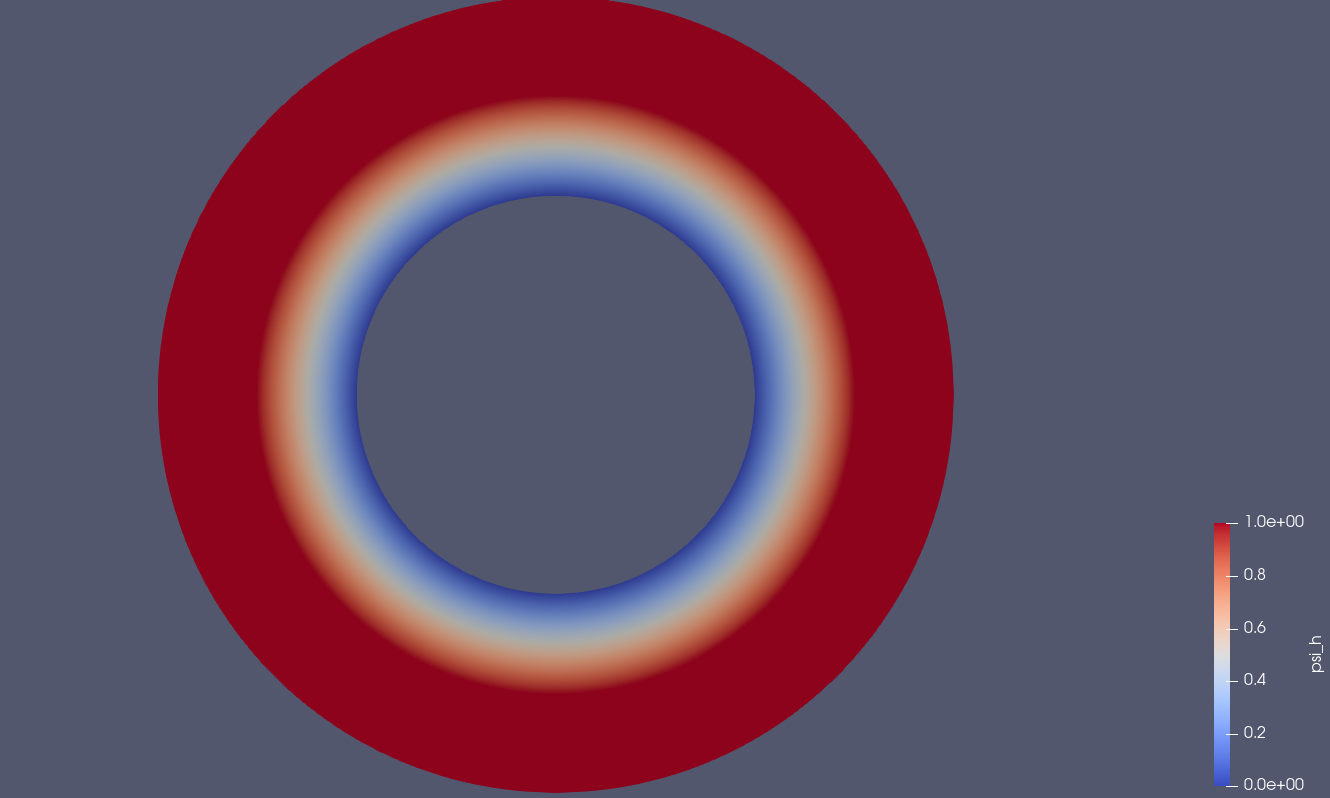
\includegraphics[width=10cm]{plot_files/manufactured_inner_curve/psi_h.png}
    \caption{A possible choice of $\psi$ on an annulus. $\Gamma$ is here in the 
    middle of the annulus. $\psi = 0$ at the inner boundary and $\psi=1$ 
    at $\Gamma$ and between $\Gamma$ and the outer boundary}
    \label{fig:psi_annulus}
\end{figure}

Then we choose $\psi$ as a simple interpolation from the inner boundary to 
the curve $\Gamma$ i.e. in logical coordinates 
\begin{align}
    \psi(\hat{x}_1,\hat{x}_2) = \begin{cases}
        2 \hat{x}_1 & \text{ for $\hat{x}_1 \leq 0.5$} 
        \\ 1 & \text{ else}.
    \end{cases}\label{eq:linear_interpolation_psi}
\end{align}This fulfills all the criteria we had for $\psi$ for this given $\Gamma$ 
(see Fig.\,\ref{fig:psi_annulus}). 

For the implementation we are using the PSYDAC library (\url{https://github.com/pyccel/psydac}) 
which is an open source 
Python 3 library 
for isogeometric analysis (see \cite{psydac_paper} for more details).
See Fig.\,\ref{fig:biot_savart_annulus_plot} for the solution where 
we chose $64$ cells for our grid on the reference domain in both dimensions and $p=2$. Note 
that $p=2$ refers to the choice of our spaces from
(\ref{eq:discrete_spline_reference_spaces}) and hence the spline space for approximating 
the magnetic field will be $\mathbb{S}_{2,1} \times \mathbb{S}_{1,2}$ 
so the lower spline degree will be one. 
The pushforward spline space achieves then an approximation error 
of $h^{p+1}$ \cite[Ch.4, (4.48)]{splines_and_pdes} if the solution is at least 
$H^{p+1}$-regular.
Thus the expected rate of 
convergence is two in our case which can be observed 
(see Fig.\,\ref{fig:convergence_analysis_biot_savart}).

\begin{figure}
    \centering
    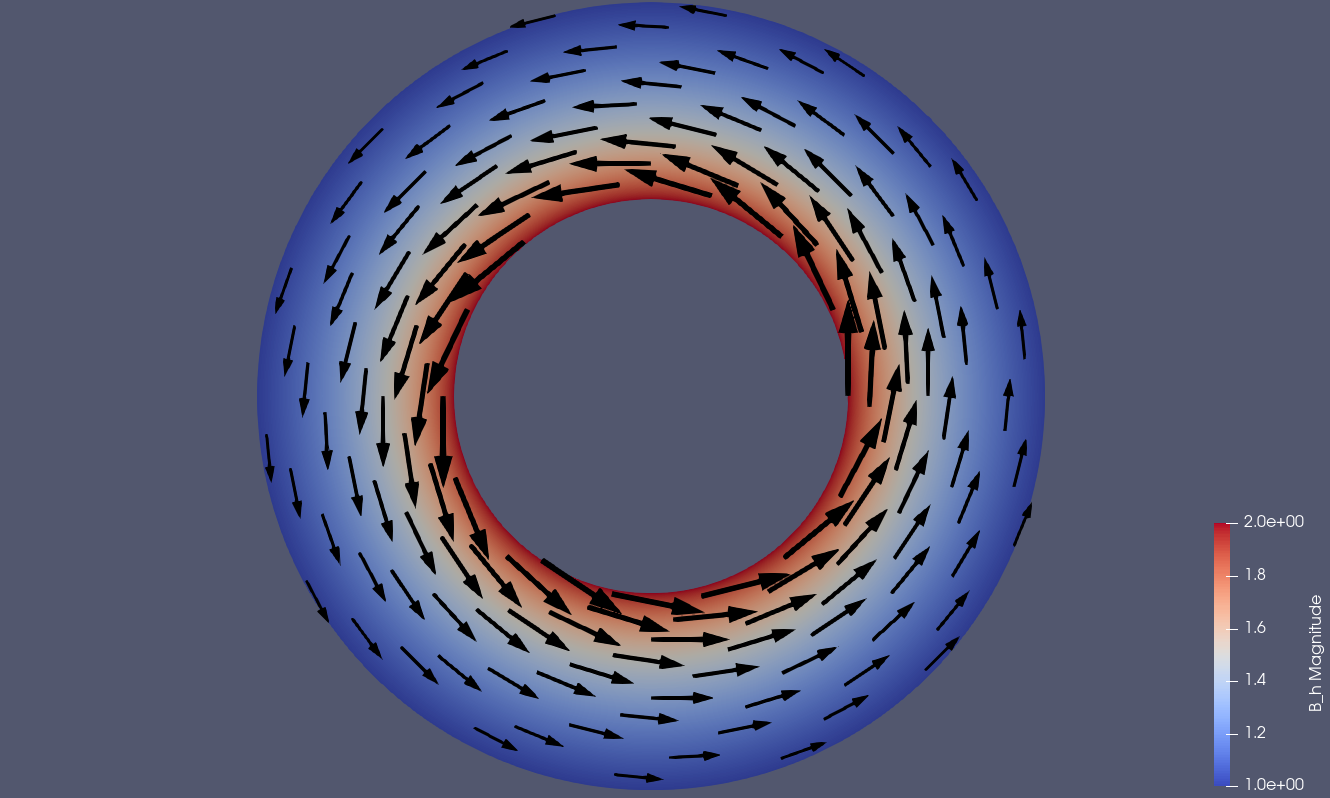
\includegraphics[width=10cm] {plot_files/biot_savart_annulus/B_h.png}
    \caption{Solution of magnetostatic problem induced by a wire through the origin in $z$-direction 
    on an annulus for 
    $64$ grid cells on the reference domain in both dimensions and spline degree $p=2$  }
    \label{fig:biot_savart_annulus_plot}
\end{figure}
{\color{red} Maybe Different curves for Biot Savart ?}
\pgfplotstableset{
    create on use/n_cells/.style={create col/copy column from table={l2_error_data/biot_savart_annulus/n_cells.csv}{0}}
}
\begin{figure}
\centering
\begin{tikzpicture}[scale=0.7]
    \begin{loglogaxis}[
        xlabel=$N$,
        ylabel=$L^2$ error,
        legend entries={$L^2$ error, $0.1\times 1/N^2$},
        xtick={8,16,32,64},
        xticklabels={$2^3$,$2^4$,$2^5$,$2^6$}
    ]

    \addplot table [x=n_cells, y index=0] {l2_error_data/biot_savart_annulus/l2_error.csv};
    \addplot [
        domain=8:100,
        samples=50,
        dashed
    ]
        {0.1 * 1/x^2};
    \end{loglogaxis}
\end{tikzpicture}
\qquad
\begin{tikzpicture}[scale=0.7]
    \begin{loglogaxis}[
        xlabel=$N$,
        ylabel=$L^2$ error,
        legend entries={$L^2$ error, $100 \times 1/N^2$},
        xtick={8,16,32,64},
        xticklabels={$2^3$,$2^4$,$2^5$,$2^6$}
    ]

    \addplot table [x=n_cells, y index=0] {l2_error_data/biot_savart_distorted/l2_error.csv};
    \addplot [
        domain=8:100,
        samples=50,
        dashed
    ]
        {100/x^2};
    \end{loglogaxis}
\end{tikzpicture}

\caption{Convergence analysis for the approximation of the Biot-Savart solution with $p=2$
    on the annulus domain (left) and the distorted annulus domain (right)
}
\label{fig:convergence_analysis_biot_savart}
\end{figure}

Now we will change the domain where the problem is posed, but we will 
stick to the Biot-Savart setting. This means we still assume the wire 
goes through the origin in $z$-direction, which results in the same solution, 
but we will approximate
on a "distorted annulus" using the same reference domain, but the different mapping 
\begin{align*}
    \mathbf{F}(\hat{x}) = \begin{pmatrix}
        (\cos^2(\hat{x}_2 ) + 1 )(\hat{x}_1 + 1)\cos(\hat{x}_2 ) 
        \\ (\cos^2(\hat{x}_2 ) + 1 ) (\hat{x}_1 + 1)\sin(\hat{x}_2 ) 
    \end{pmatrix}.
\end{align*}
which results in a kind of "distorted annulus"(see \ref{}). 

Note that now for this domain we do not have 
the homogeneous boundary condition
$\mathbf{B}\cdot \mathbf{n} = 0$ anymore. Thus we have to deal with the boundary conditions 
by using a standard lifting approach which means we take an interpolation of the boundary conditions 
$\mathbf{B}_{h,g}$ which we compute before and then split
$\mathbf{B}_{h} = \mathbf{B}_{h,0} + \mathbf{B}_{h,g}$ with $\mathbf{B}_{h,0}\in V_h^1$.
Then we substitute $P_h^1 \mathbf{B}_h$ in 
(\ref{eq:system_with_penalties:eq1})-(\ref{eq:system_with_penalties:eq3}) 
with $\mathbf{B}_{h,0} + \mathbf{B}_{h,g}$ and put the terms with  
$\mathbf{B}_{h,g}$ on the right hand side. 
This leads to the same left hand side, but as right hand side we get
$-\langle J, \tau_h \rangle + \langle \mathbf{B}_{h,g}, \veccurl \tau_h \rangle$ in 
the first equation, $-\langle\diver  \mathbf{B}_{h,g} ,\diver \mathbf{v}_{h} \rangle$
in the second and $C_1 - \langle\veccurl \psi,\mathbf{B}_{h,g} \rangle$ 
in the third. In practice, since we know the exact solution $\mathbf{B}$ we simply take 
$\mathbf{B}_{h,g} \vcentcolon= (I-P^1_h)\mathbf{B}$. The remaining steps of assembling 
the system are completely analogous to Sec.\,\ref{sec:assembling_the_discrete_system}. 


As $\psi$ we use the exact same definition as in (\ref{eq:linear_interpolation_psi}) 
which results in a different 
curve due to the different domain parametrization (see Fig.\,\ref{fig:psi_distorted_annulus}). $J$ is of course
still zero and the curve integral does not change either. We obtain again 
second order convergence for $p=2$ (see Fig.\ref{fig:convergence_analysis_biot_savart}), 
but the error is several orders of magnitude larger compared to the normal annulus. 

\begin{figure}
    \centering
    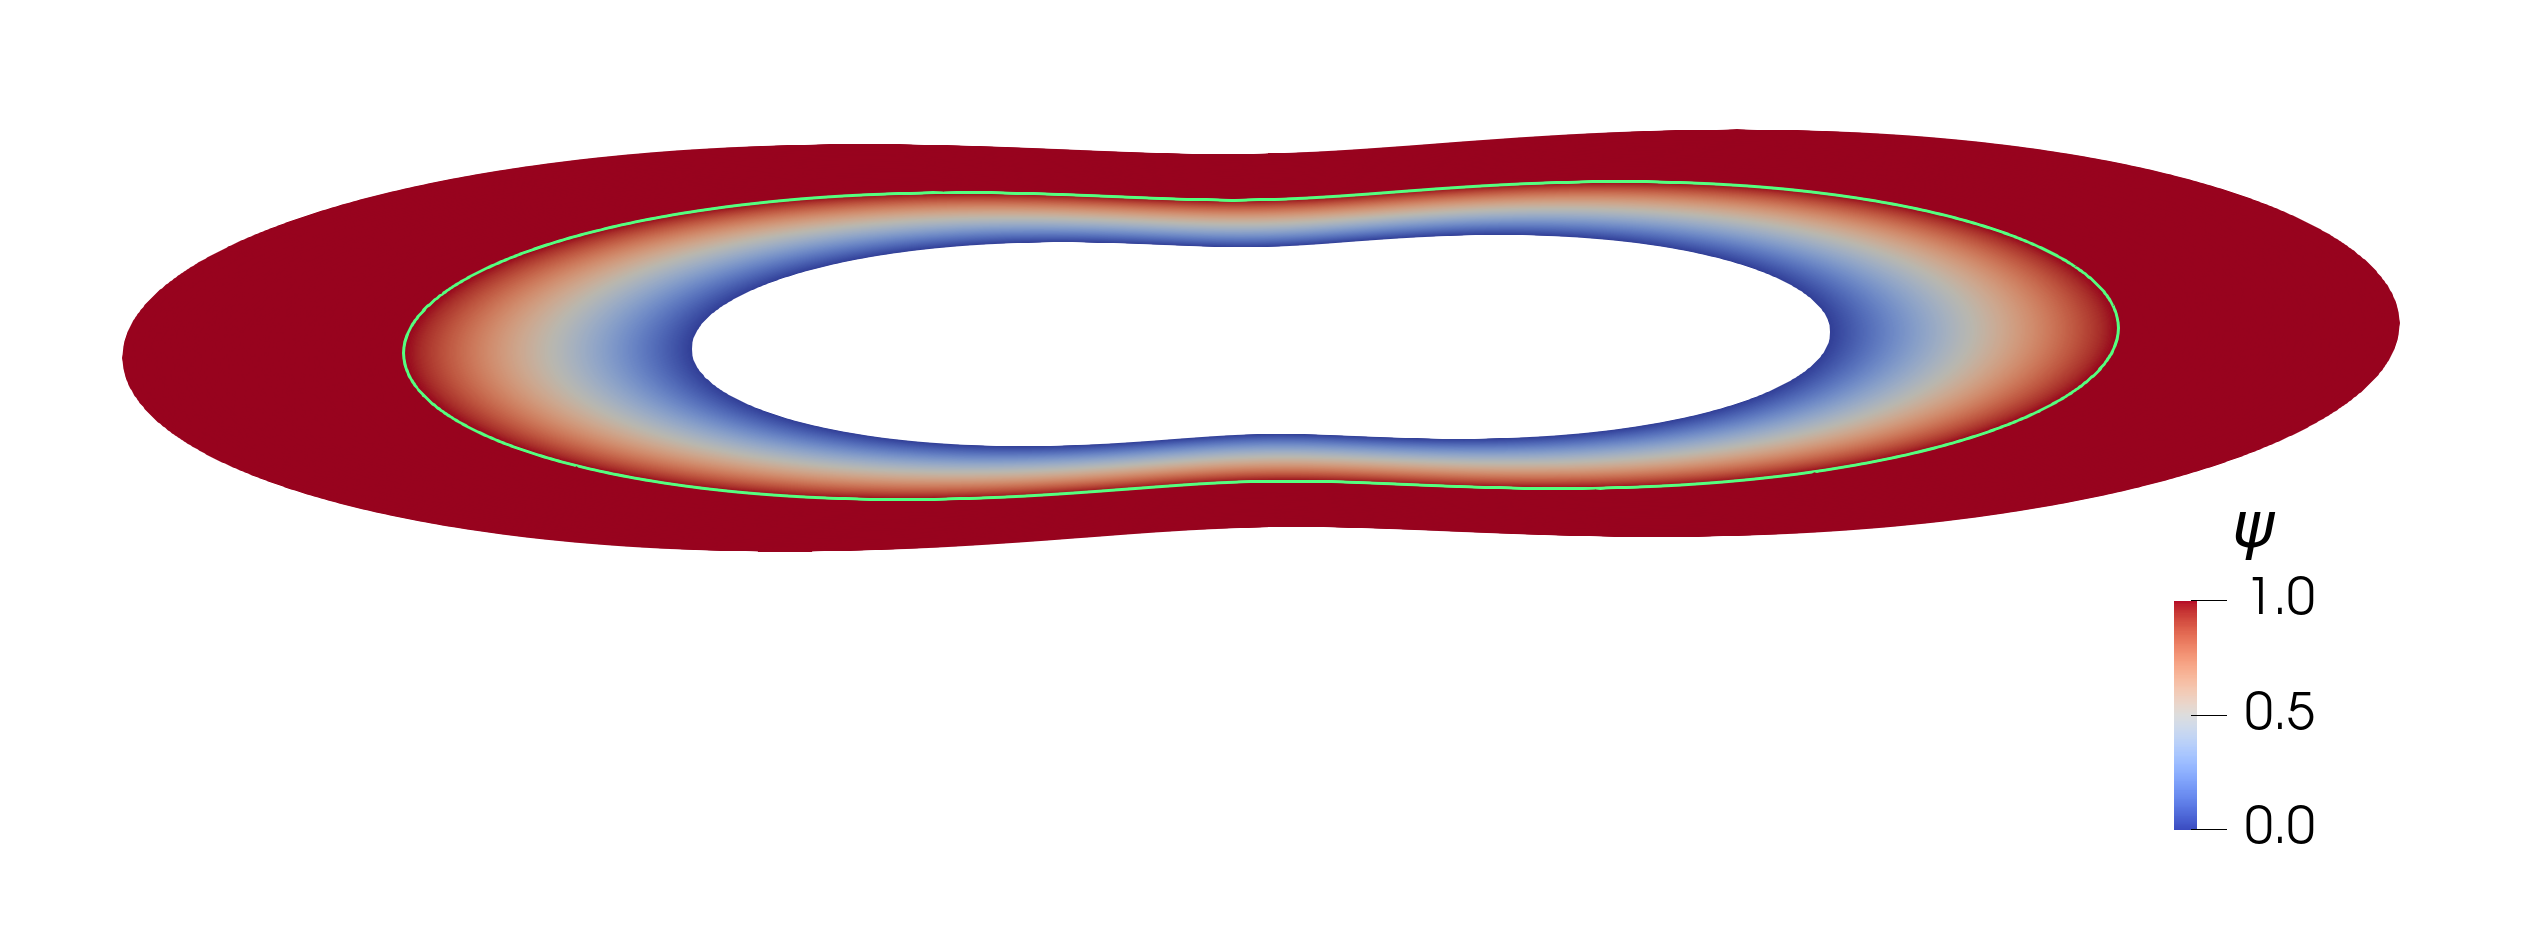
\includegraphics[width=10cm]{plot_files/biot_savart_distorted/psi_h.png}
    \caption{$\psi$ on the distorted annulus domain. $\Gamma$ is again 
        in the middle between the interior and exterior boundary.
    }
    \label{fig:psi_distorted_annulus}
\end{figure}
\begin{figure}
    \centering
    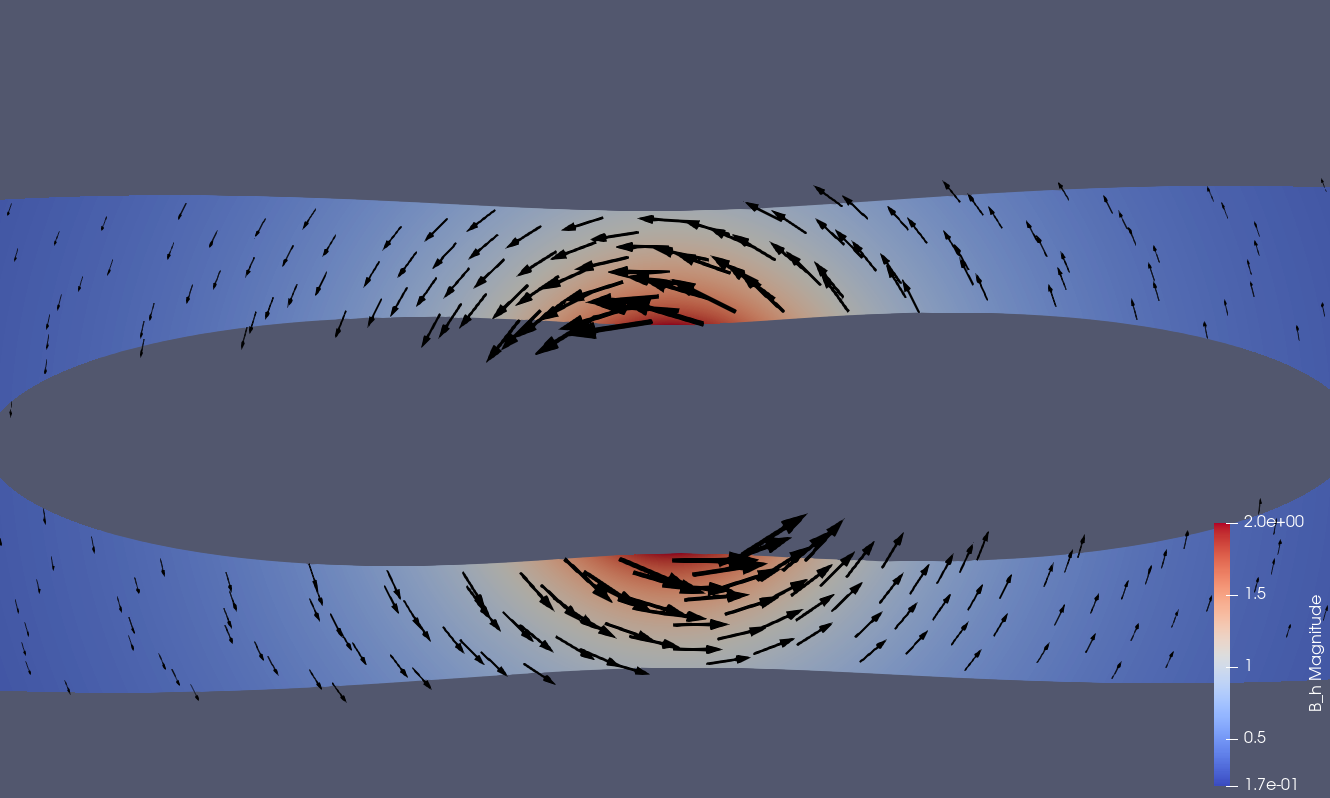
\includegraphics[width=10cm]{plot_files/biot_savart_distorted/B_h.png}
    \caption{Solution of the Biot-Savart law on the distorted annulus 
    with $64$ cells in both dimensions and $p=2$. The wire 
    is in the centre pointing towards the point of view.
    }
    \label{fig:distorted_annulus_plot}
\end{figure}

\subsection{Manufactured solution}

As an example with a non-vanishing $J$, we will use a manufactured solution. 
Let $\mathbf{B}(x) = (|x|^2 -2) (-x_2,x_1)^\top$. It is easy to see that 
$\diver \mathbf{B} = 0$ and 
$\mathbf{B}\cdot \mathbf{n} = 0$ for the annulus. 
This results in   
\begin{align*}
    J(x) = 4 |x|^2 - 12 |x| + 8.
\end{align*}
We will pose this problem on the annulus domain from before, but we will use two 
different choices for $\Gamma$. 
$\Gamma_1$ will be the same $\Gamma$ as before, but $\Gamma_2$ will 
be the outer boundary of $\Omega$ i.e. 
it is equal to $\partial\Omega_{out}$. 
Since $J$ is not zero this leads to different curve integrals
\begin{align*}
    \int_{\Gamma_1} \mathbf{B}\cdot d\ell = \frac{9\pi}{8} \quad \text{  and  } \quad
    \int_{\Gamma_2} \mathbf{B}\cdot d\ell = 0.
\end{align*}
For $\Gamma_1$ we will choose $\psi$ as before and for $\Gamma_2$ we take
$\psi$ as the solution of the Laplace problem with boundary condition 
$\psi=0$ on $\partial\Omega_{in}$ and $\psi=1$ on $\partial\Omega_{out}$
(see Fig.\,\ref{fig:psi_poisson}). We observe the same convergence rate 
(Fig.\,\ref{fig:convergence_analysis_manufactured}).

\begin{figure}
    \centering 
    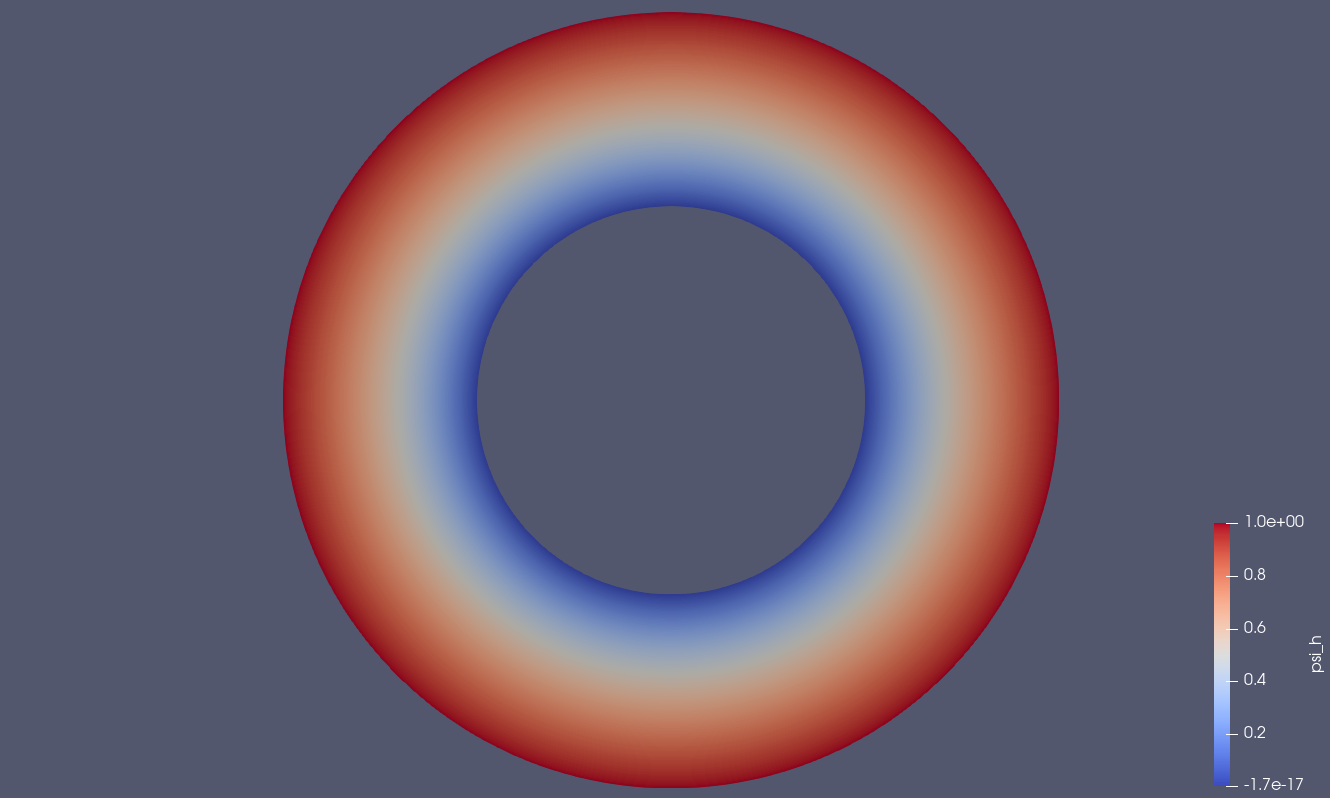
\includegraphics[width=10cm]{plot_files/manufactured_poisson_psi/psi_h.png}
    \caption{$\psi$ as the solution of a Poisson problem with $\psi=0$ 
    on the interior and $\psi = 1$ on the exterior boundary. $\Gamma$ 
    is here equal to $\partial \Omega_{out}$.}
    \label{fig:psi_poisson}
\end{figure}

\begin{figure}
    \centering
    \begin{tikzpicture}[scale=0.8]
        \begin{loglogaxis}[
            xlabel=$N$,
            ylabel=$L^2$ error,
            legend entries={$\Gamma=\Gamma_1$, $\Gamma=\Gamma_2$, $0.1\times 1/N^2$},
            xtick={8,16,32,64},
            xticklabels={$2^3$,$2^4$,$2^5$,$2^6$}
        ]
    
        \addplot table [x=n_cells, y index=0] {l2_error_data/manufactured_inner_curve/l2_error.csv};
        \addplot table [x=n_cells, y index=0] {l2_error_data/manufactured_poisson_psi/l2_error.csv};
        \addplot [
            domain=8:100,
            samples=50,
            dashed
        ]
            {0.1 * 1/x^2};
        \end{loglogaxis}
    \end{tikzpicture}
    \caption{Convergence analysis for the manufactured solution $\mathbf{B}(x) = (|x|^2 -2) (-x_2,x_1)^\top$
        with different choices of $\psi$ corresponding to different curves $\Gamma_1$ (as before) and
        $\Gamma_2$ (equal to the exterior boundary).
    }
    \label{fig:convergence_analysis_manufactured}
\end{figure}    
\end{document}